\documentclass[aspectratio=169]{beamer}
\usetheme{Boadilla}
\usepackage[utf8]{inputenc}       % Codificação de entrada
\usepackage[T1]{fontenc}          % Codificação de saída
\usepackage[portuguese]{babel}   % Idioma
\usepackage{XCharter}             % Fonte principal
\AtBeginDocument{\fontsize{12}{12}\selectfont}

%\usepackage{geometry}
%\geometry{papersize={210mm,150mm}}

\usepackage{color}
\usepackage{graphicx}
\usepackage{amsmath, amssymb, amsfonts}
\usepackage{bm}
\usepackage{booktabs}
\usepackage{multirow}
\usepackage{caption}
\usepackage{subfigure}
\usepackage{wrapfig}
\usepackage{multicol}
\usepackage{sidecap}
\usepackage{tikz}
\usepackage{listings}
\usepackage{siunitx}
\usepackage{pdfpages}
\usepackage{float}
\usepackage{hyperref}
\usepackage{academicons}
\usepackage{setspace}

\newcommand{\eng}[1]{\textsl{#1}}
\newcommand{\cod}[1]{\texttt{#1}}


\title[Minicurso FPGAs]{\huge Hardware Reconfigurável}

\author[Prof. Dr. Oscar Eduardo Anacona Mosquera]{Prof. Dr. Oscar Eduardo Anacona Mosquera \newline\newline 
\scriptsize{oscar.mosquera@ufmt.br}
}

\AtBeginSection[]
{
	\begin{frame}{Conteúdo}
		\tableofcontents[currentsection]
	\end{frame}
}
\begin{document}

%%====================================================================================
\begin{frame}[plain]
\titlepage
\end{frame}
%%====================================================================================
\section{Objetivos}

%%====================================================================================
\begin{frame}
	\frametitle{Objetivos}
	
	\begin{itemize}
		\item \textbf{Fluxo de Projeto em FPGA:}
		\begin{itemize}
			\item Compreender o fluxo de projeto típico para desenvolver aplicações em FPGA.
			\item Explorar as etapas desde a especificação do projeto até a implementação e teste em hardware.
		\end{itemize}
		
		\item \textbf{FPGA: CLBs, LUTs, PIPs, IOBs:}
		\begin{itemize}
			\item Entender os componentes principais de um FPGA, incluindo Blocos de Lógica Configurável (CLBs), Tabelas de Busca (LUTs), Pontos de Interconexão Programável (PIPs) e Blocos de Entrada/Saída (IOBs).
		\end{itemize}
		
		\item \textbf{Módulos dos FPGAs Antigos e Modernos:}
		\begin{itemize}
			\item Comparar e contrastar as arquiteturas de FPGAs antigos e modernos.
			\item Identificar as melhorias e avanços nas capacidades de processamento, eficiência energética e recursos de integração.
		\end{itemize}
		
		\item \textbf{SoC-FPGA:}
		\begin{itemize}
			\item Explorar os conceitos de SoC-FPGA (System-on-Chip FPGA) e suas vantagens.
			\item Compreender como a integração de FPGA com processadores de aplicativos em um único chip permite soluções altamente integradas e flexíveis.
		\end{itemize}
	\end{itemize}

\end{frame}
%%====================================================================================

\section{Introdução}
%%====================================================================================
\begin{frame}{Classical digital design flow}
	
	
	\begin{block}{Specifications}
	\justifying
	Projete um detetor de numeros primos para valores entre $0_{10}$ a $7_{10}$.O circuito deve ser capaz de indicar um número primo com um atraso inferior a 200 ns.
	\end{block}	
	
	
	\begin{block}{Functional design}
	\justifying
	A funcionalidade e o comportamento do sistema são definidos em termos de entradas, saídas e operações necessárias para realizar uma tarefa específica. 
	\end{block}		
	
	\begin{figure}[h]
		\centering
		\includegraphics[width=0.57\textwidth]{Figs/fig05.png}
	\end{figure}
	
\end{frame}
%%====================================================================================

%%====================================================================================
\begin{frame}{Classical digital design flow}
	
	
	\begin{block}{Synthesis}
		\justifying
		Processo de transformar uma descrição de alto nível do comportamento funcional de um sistema em uma representação física ou lógica que pode ser implementada em hardware.
	\end{block}	
	
	\begin{figure}[h]
	\centering
	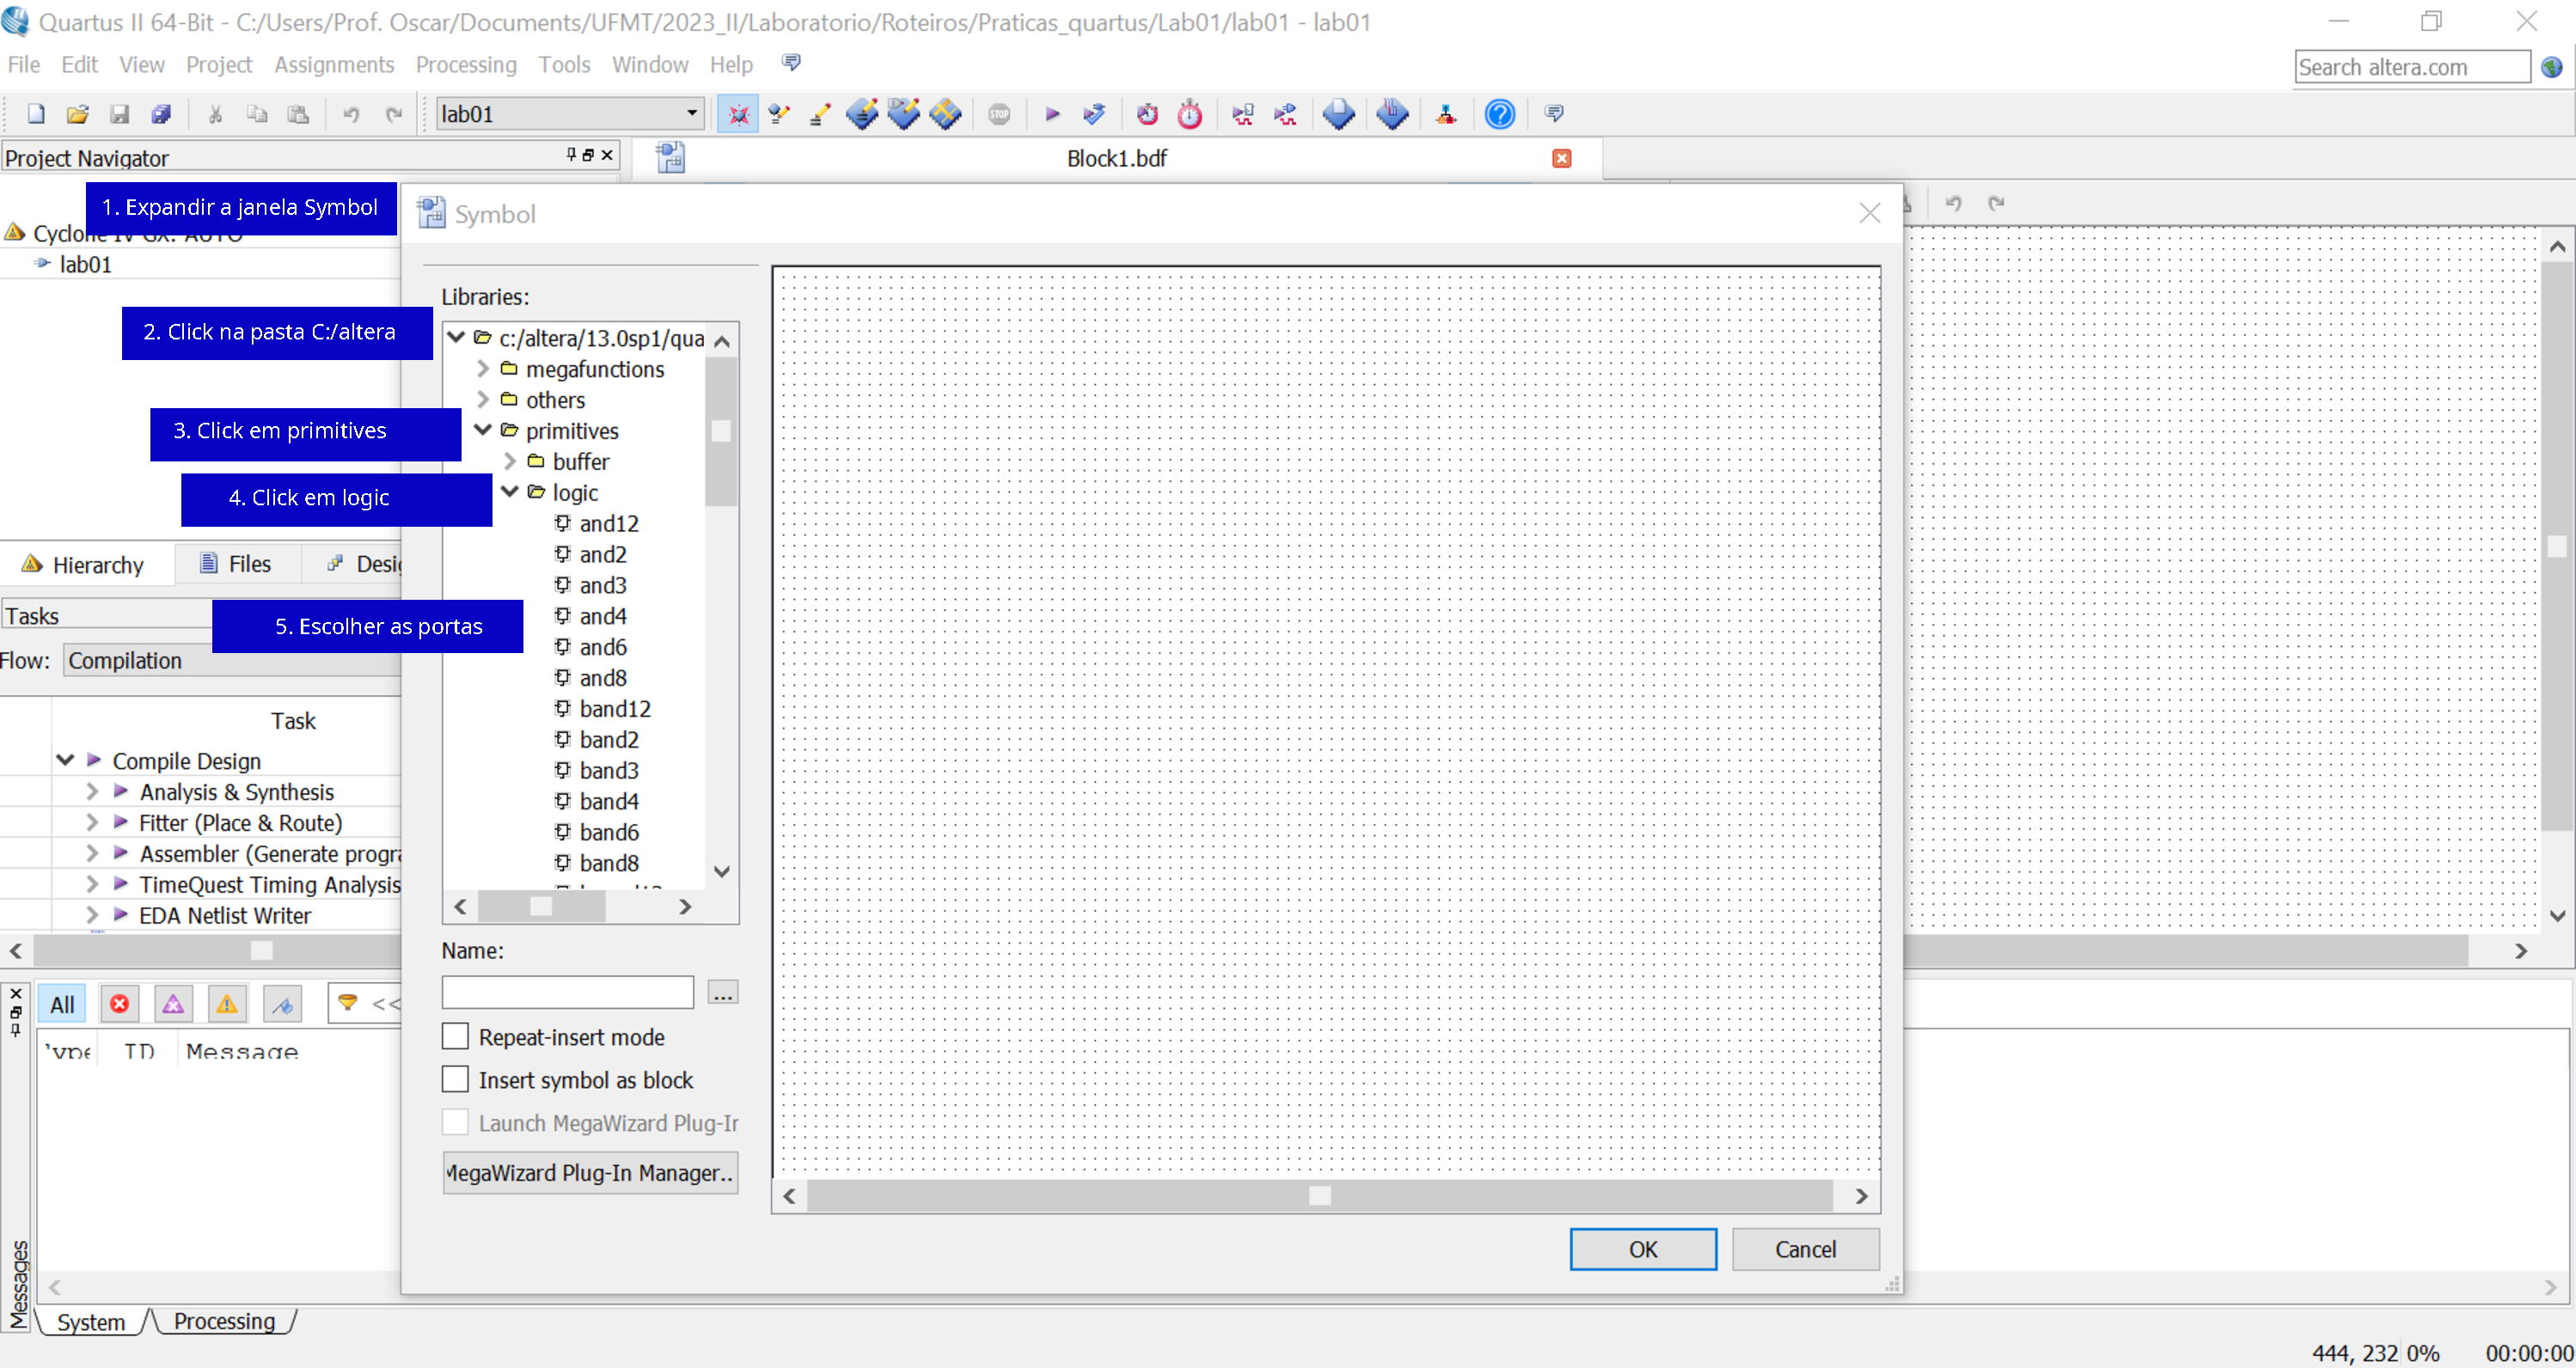
\includegraphics[width=0.57\textwidth]{Figs/fig06.png}
	\end{figure}
	
\end{frame}
%%====================================================================================



%%====================================================================================
\begin{frame}{Classical digital design flow}
	
	\begin{block}{Technology mapping}
		\justifying
		Nesta fase, a \textbf{netlist} gerada durante a síntese lógica é mapeada para os recursos específicos disponíveis no hardware de destino.
	\end{block}		
	
	\begin{figure}[h]
		\centering
		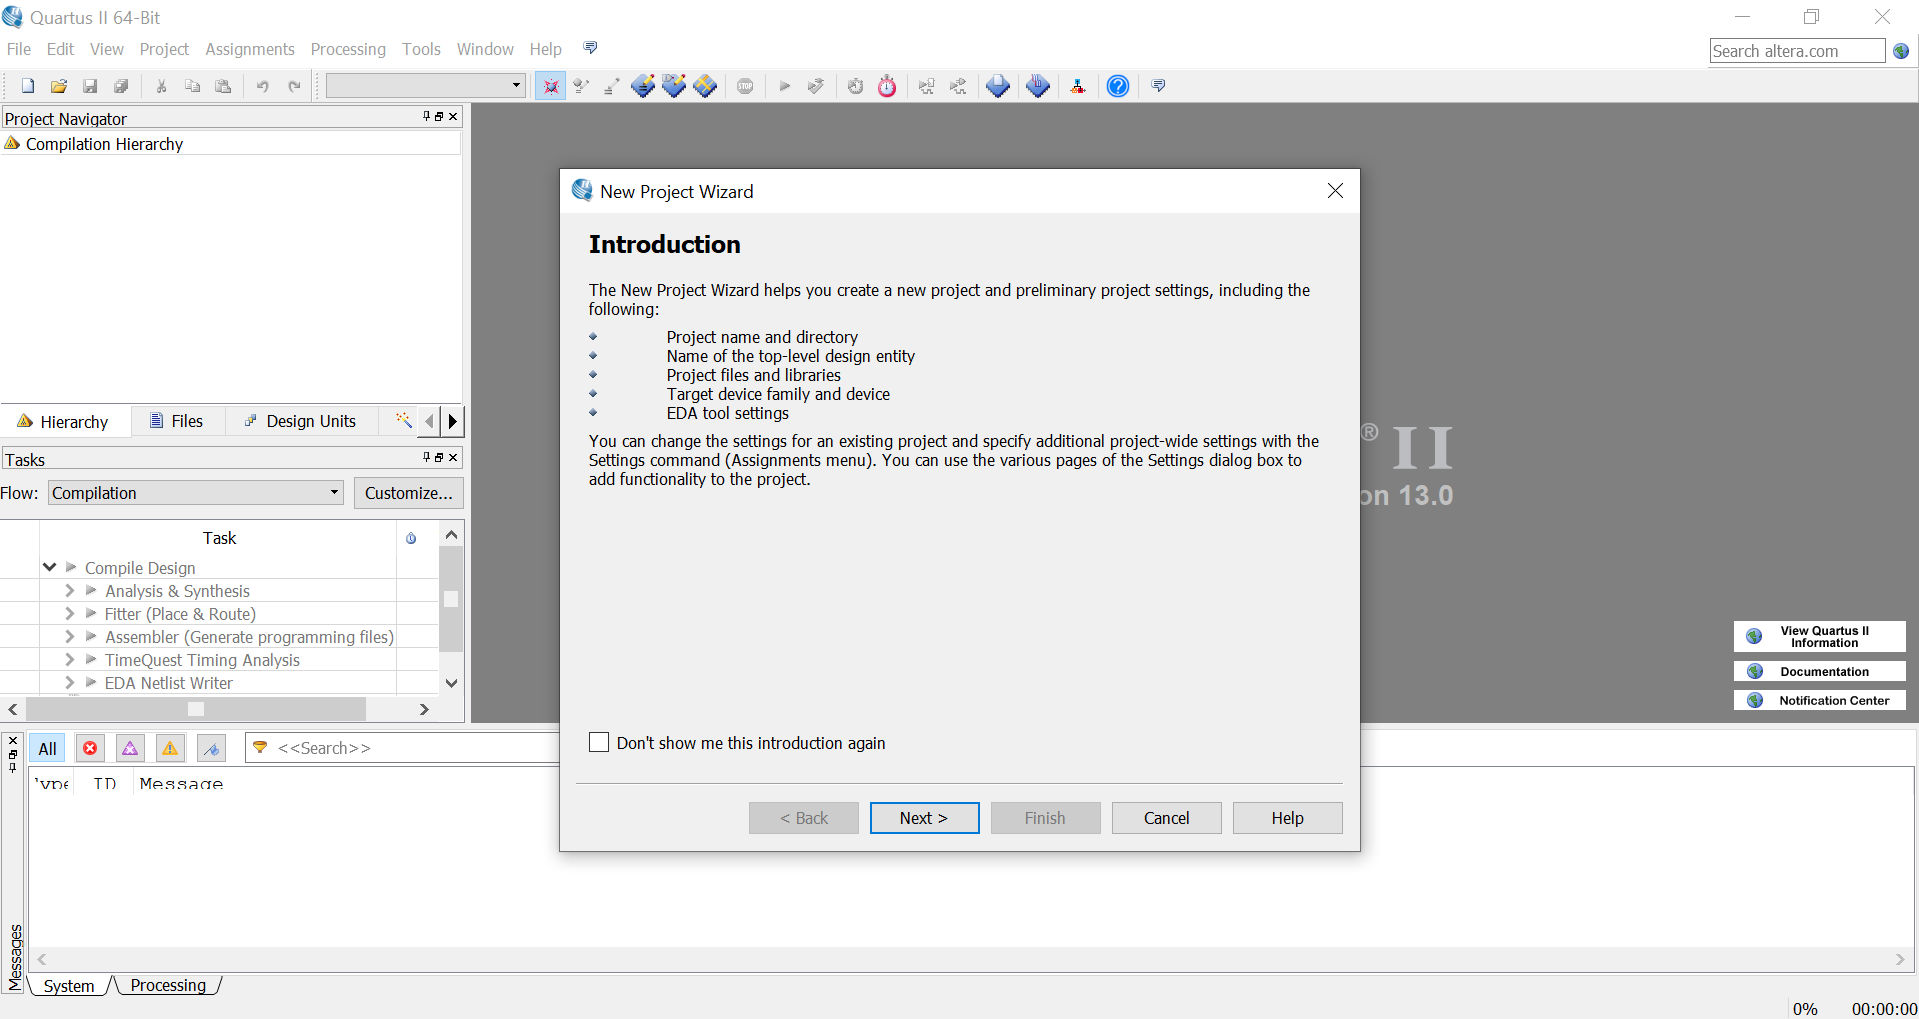
\includegraphics[width=0.57\textwidth]{Figs/fig07.png}
	\end{figure}
	
\end{frame}
%%====================================================================================

%%====================================================================================
\begin{frame}{Classical digital design flow}
	
	
	\begin{block}{Place and route}
		\justifying
		Processo de transformar uma descrição de alto nível do comportamento funcional de um sistema em uma representação física ou lógica que pode ser implementada em hardware.
	\end{block}	
	
	\begin{figure}[h]
		\centering
		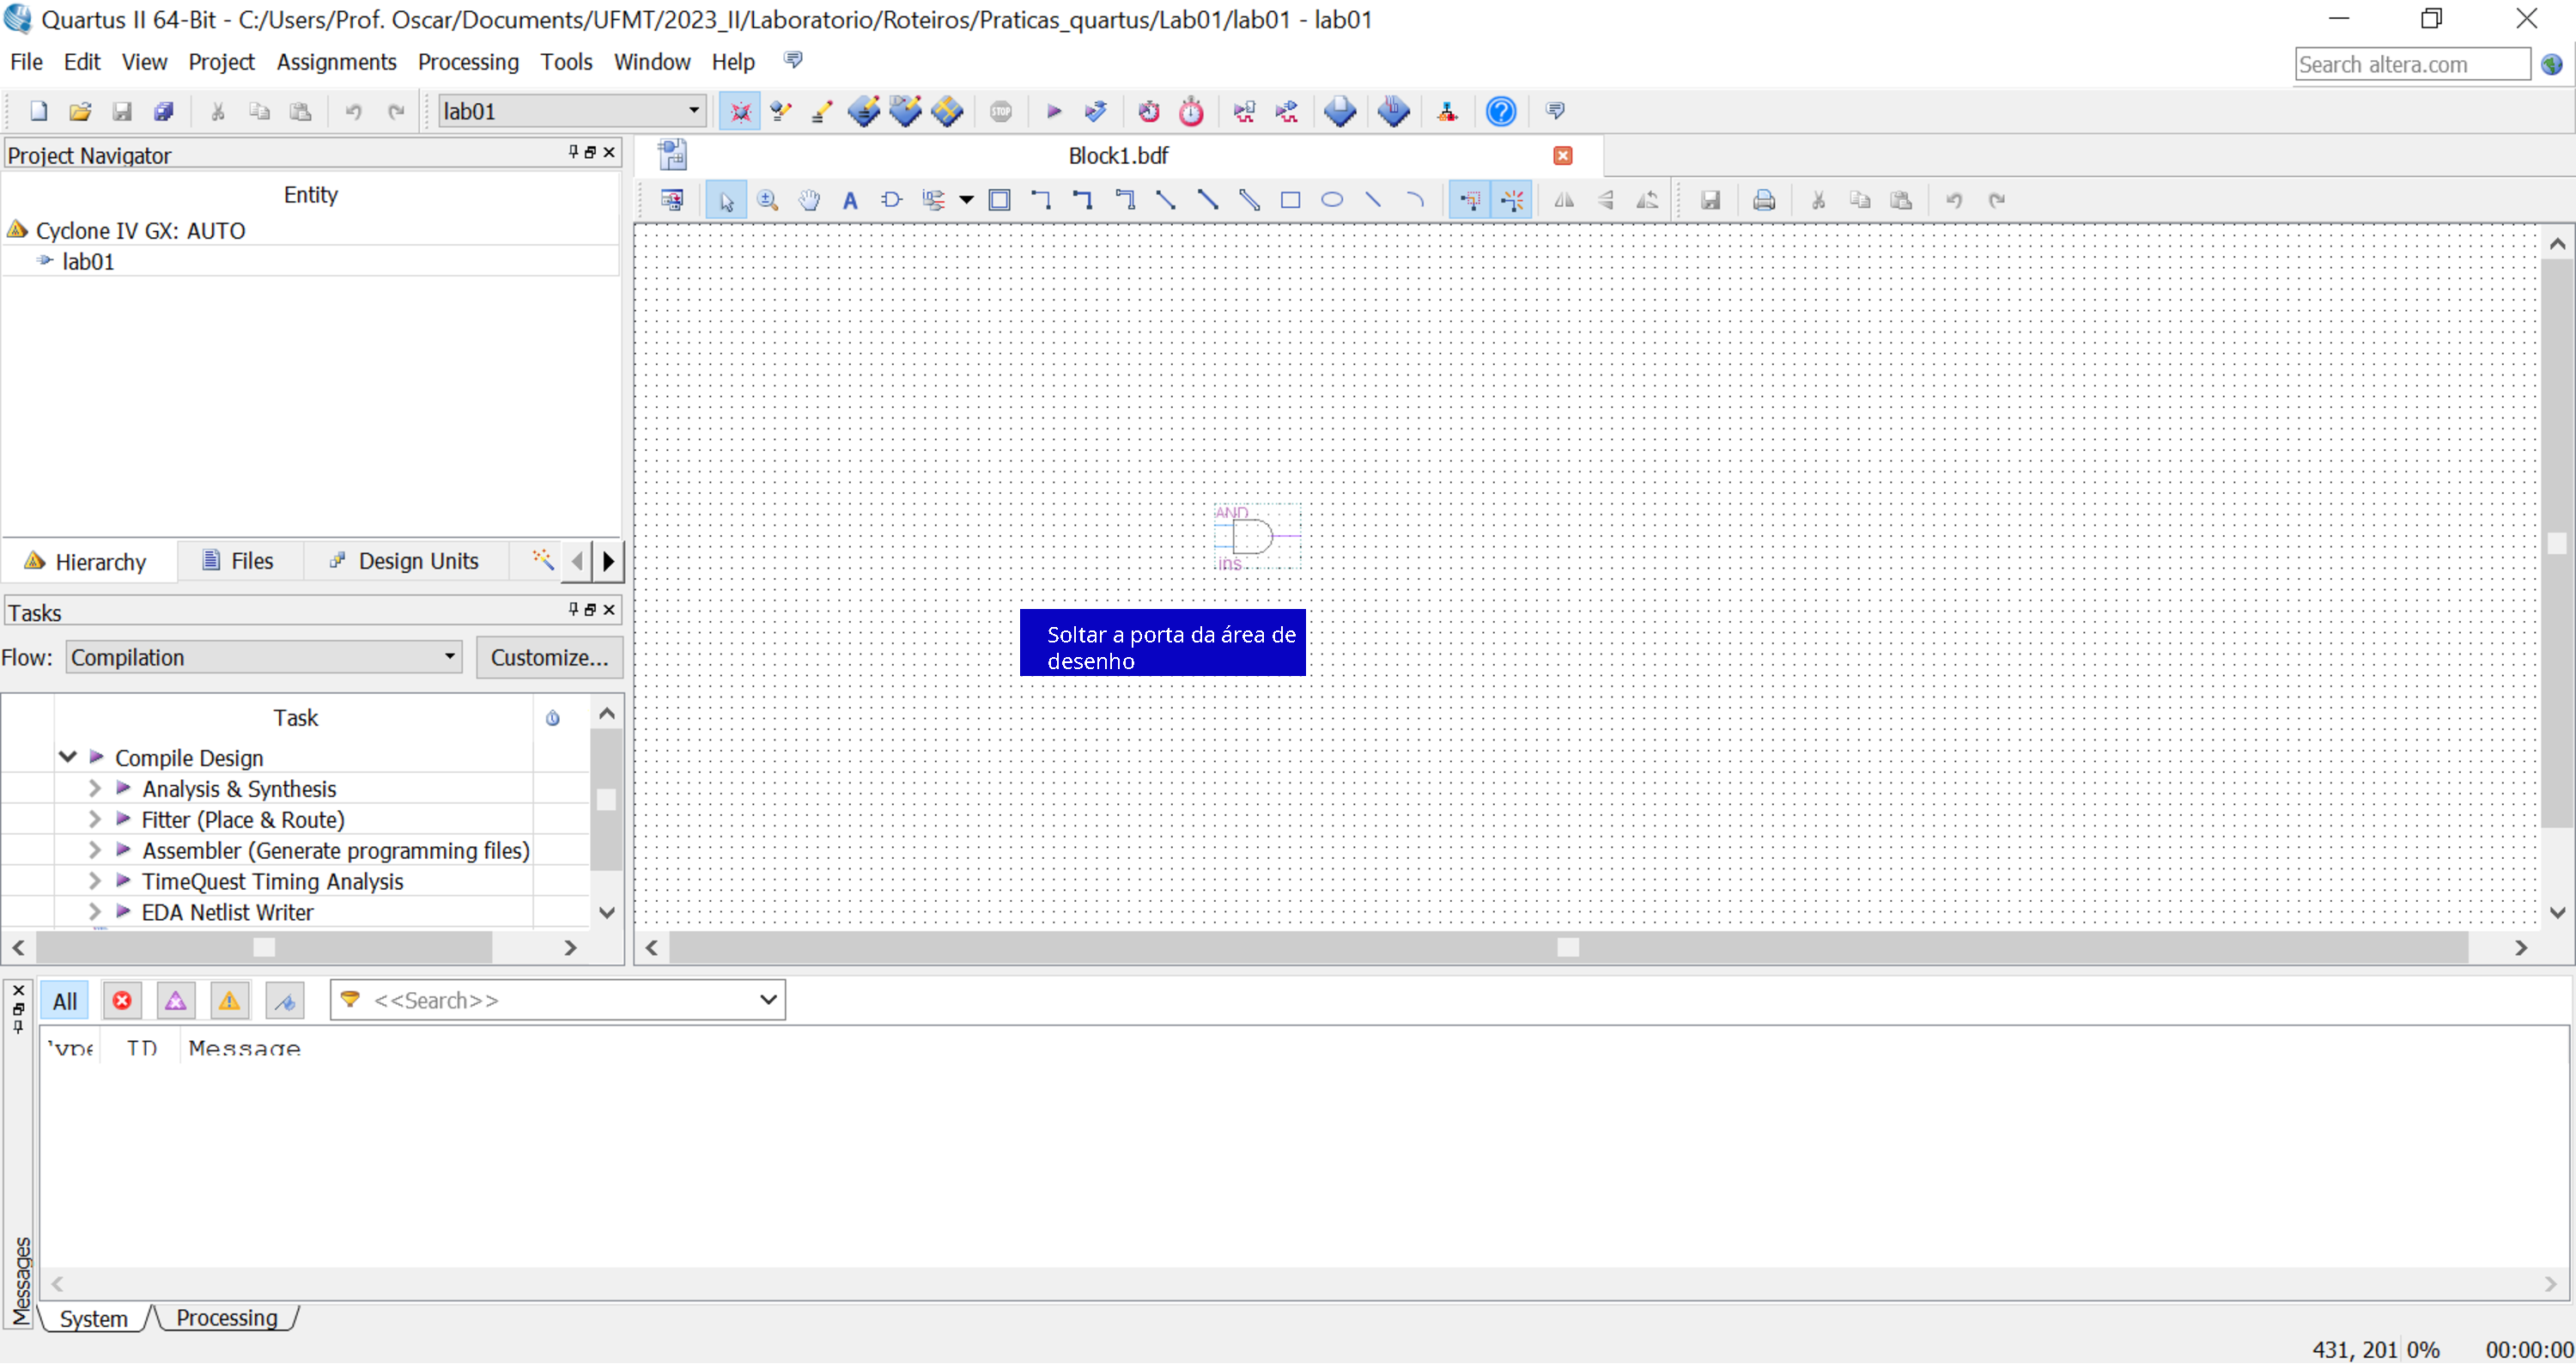
\includegraphics[width=0.27\textwidth]{Figs/fig08.png}
	\end{figure}

	
\end{frame}
%%====================================================================================
%%====================================================================================
\begin{frame}{Classical digital design flow}

	\begin{block}{Verification}
		\justifying
		Se concentra em garantir que o projeto atenda aos requisitos de funcionalidade, desempenho e confiabilidade estabelecidos durante a fase de especificação.
	\end{block}		
	
	\begin{figure}[h]
		\centering
		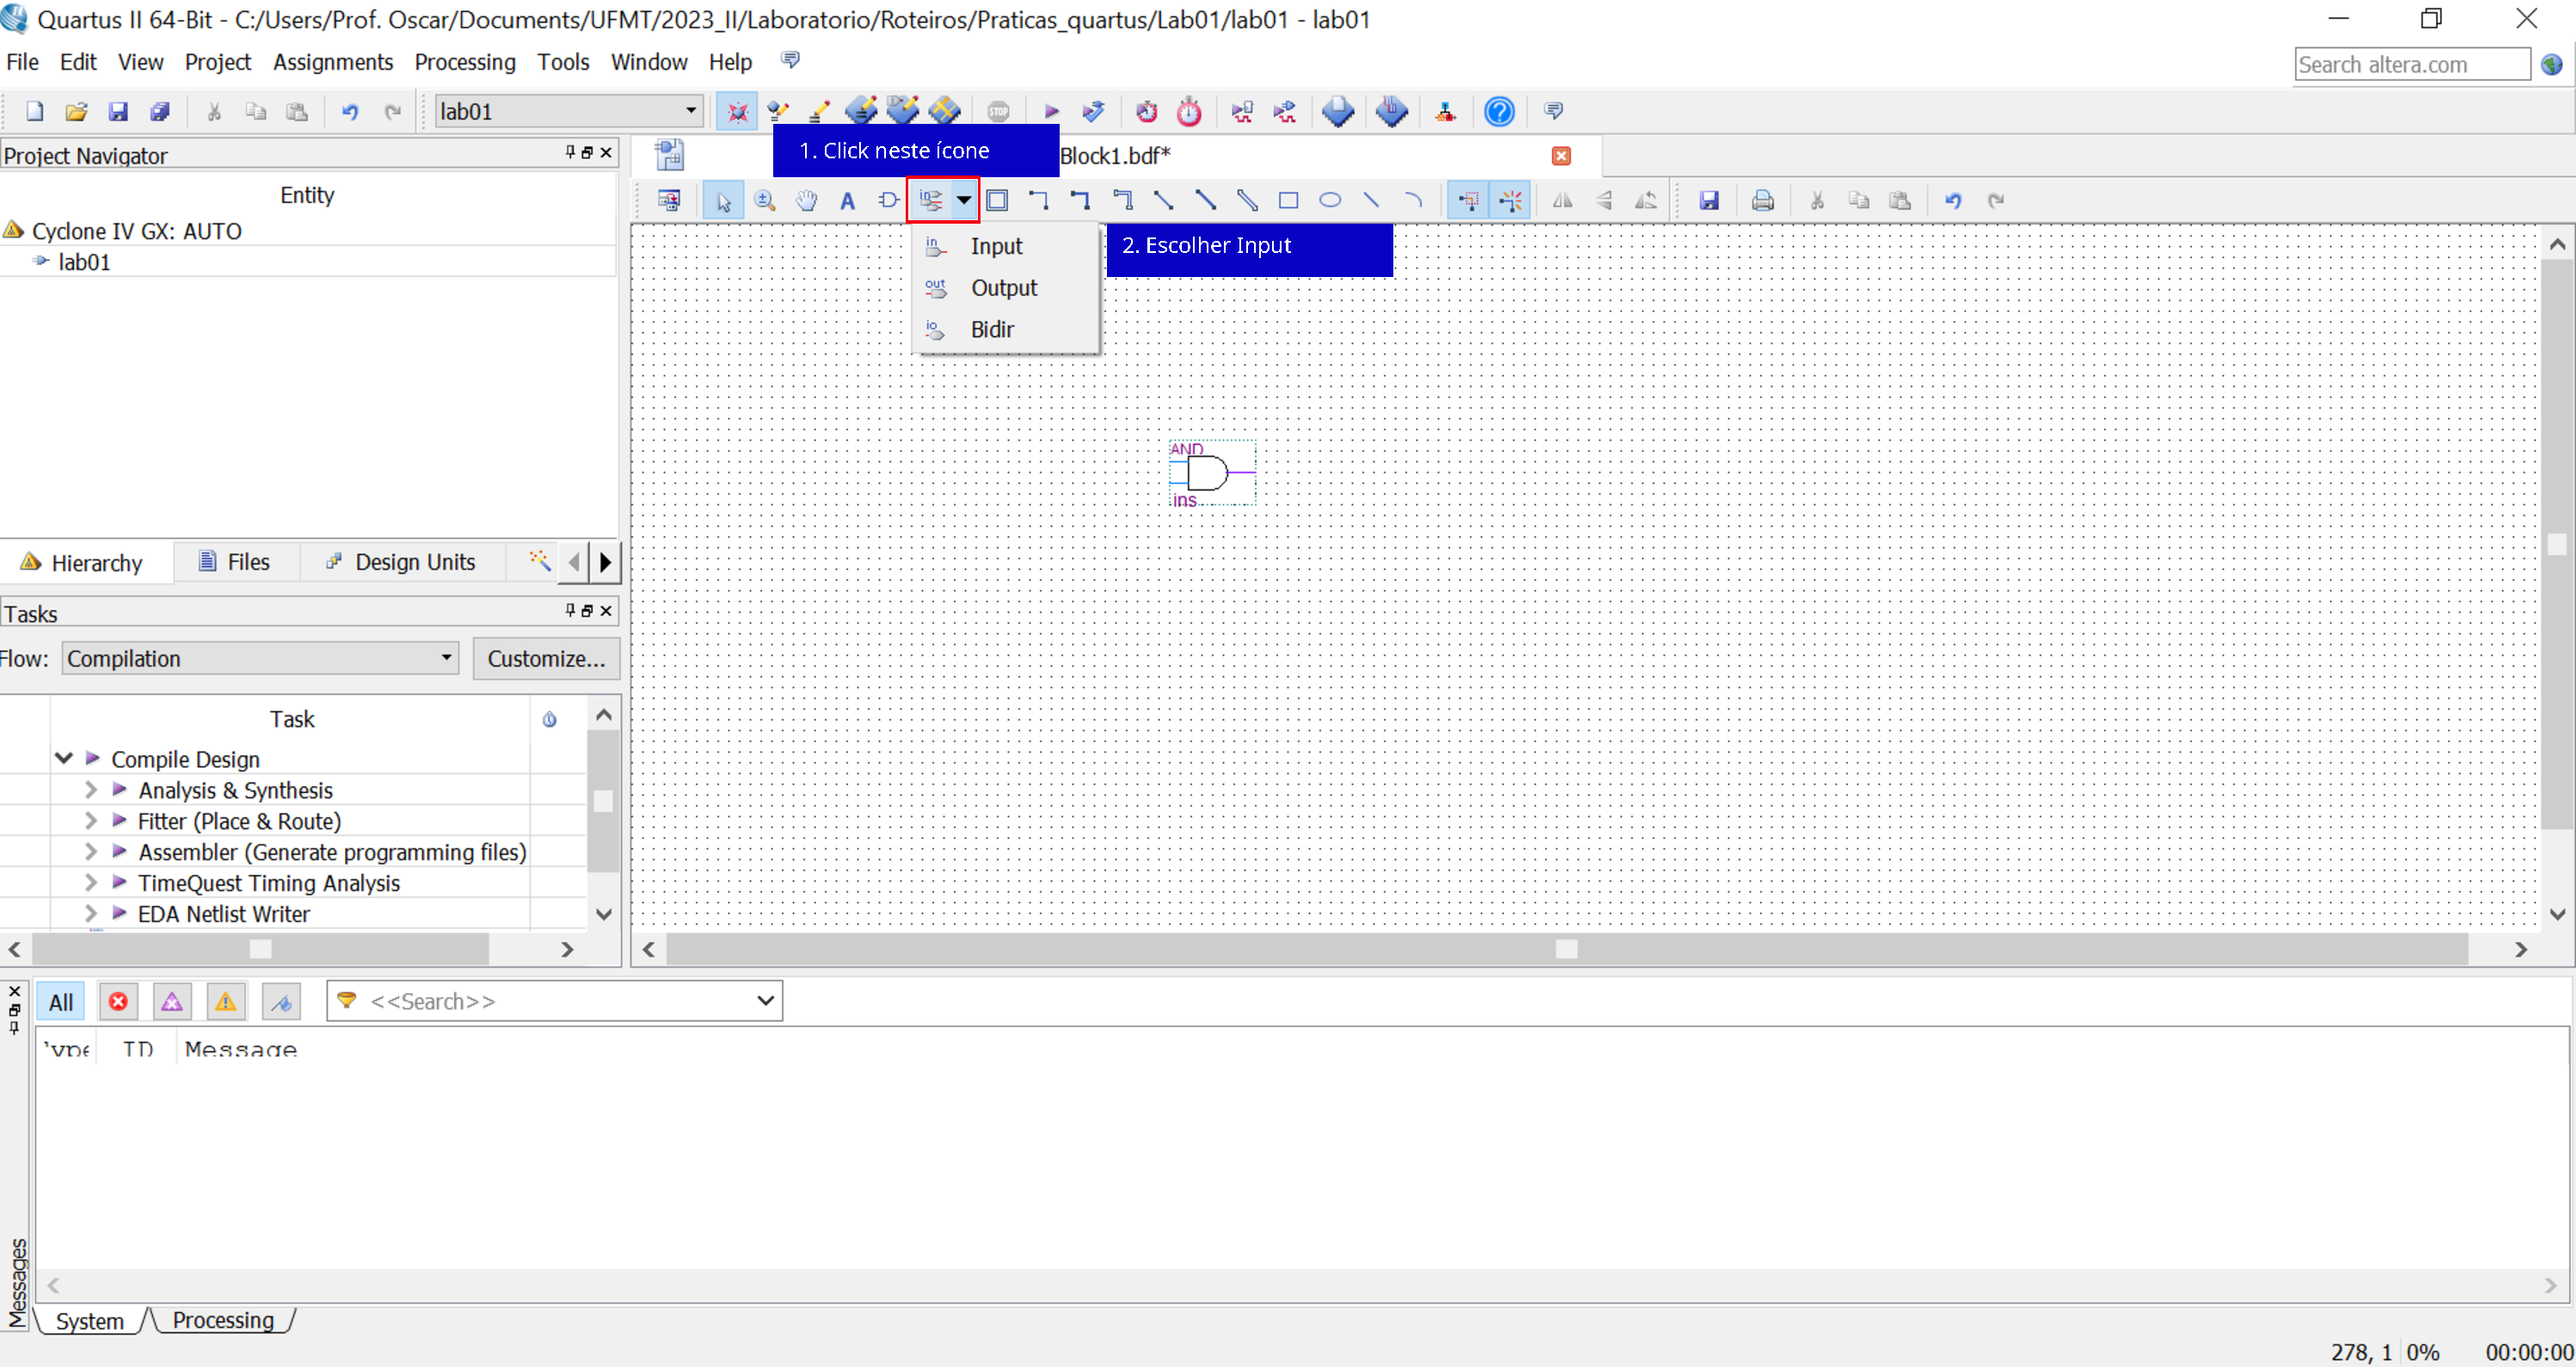
\includegraphics[width=0.57\textwidth]{Figs/fig09.png}
	\end{figure}
	
\end{frame}
%%====================================================================================

%%====================================================================================
\begin{frame}{Classical digital design flow}
	
	\begin{block}{Fabrication}
		\justifying
		O projeto em que o circuito integrado é efetivamente construído a partir do layout físico desenvolvido durante as etapas anteriores do projeto, como colocação e roteamento.
	\end{block}	
	
	\begin{figure}[h]
		\centering
		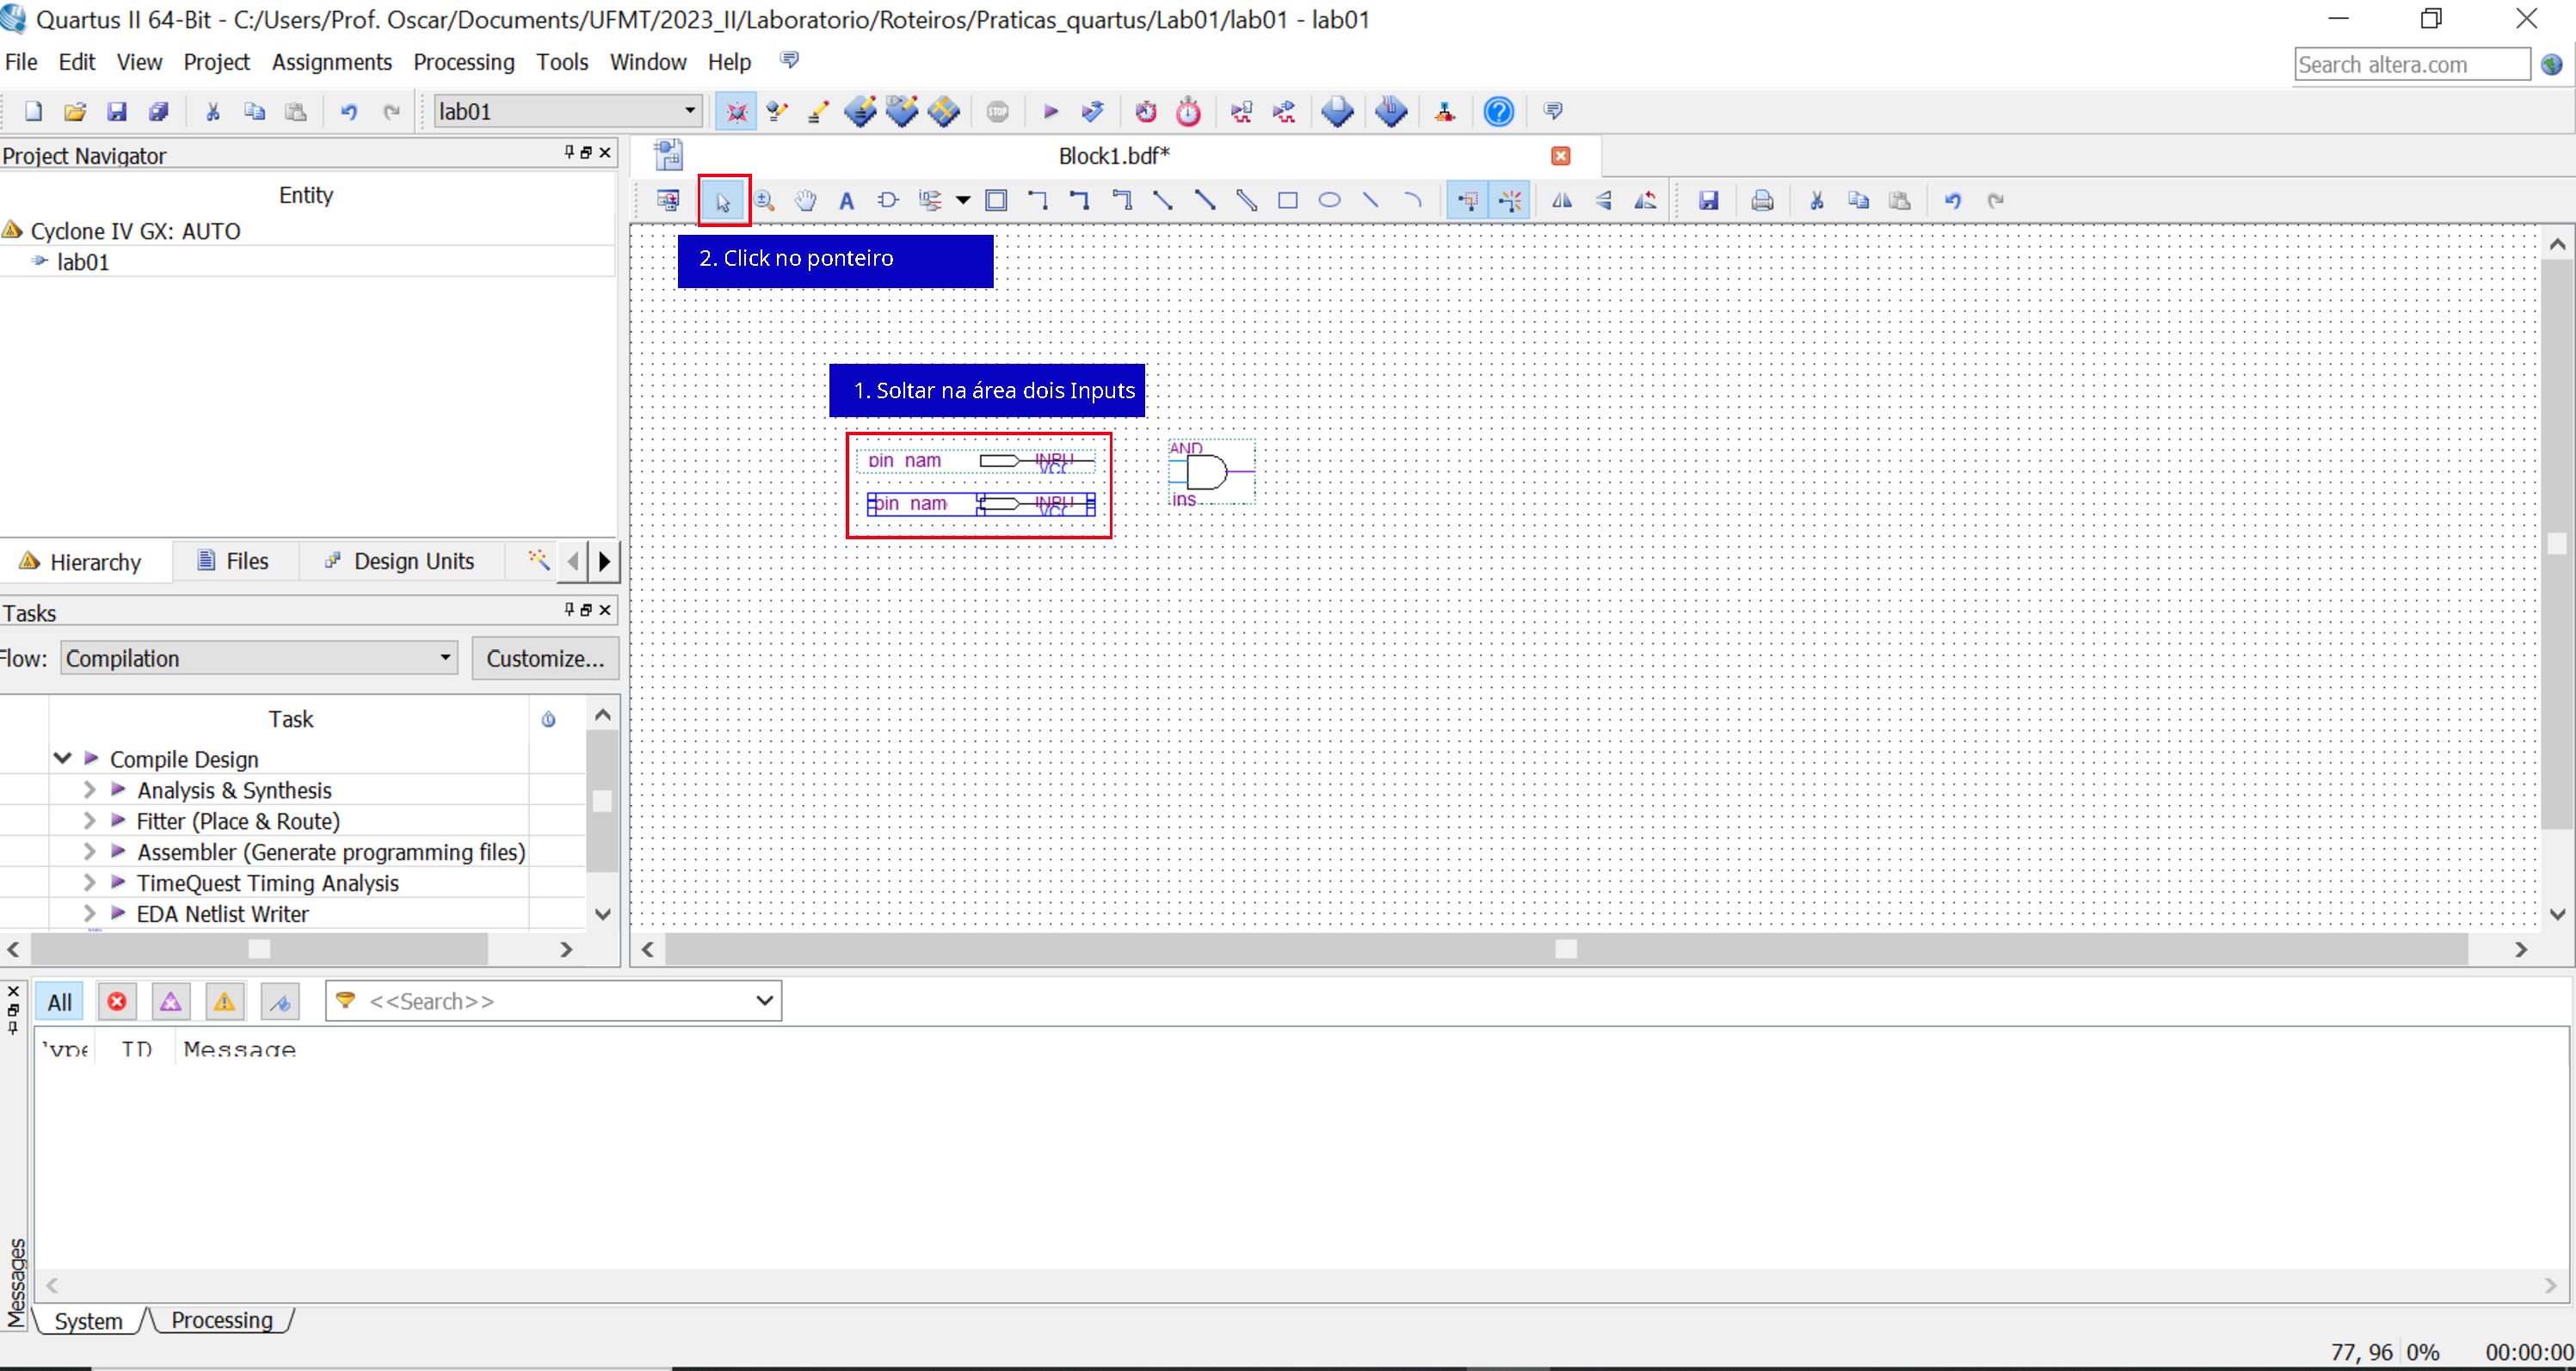
\includegraphics[width=0.67\textwidth]{Figs/fig10.png}
	\end{figure}
	
\end{frame}
%%====================================================================================

\section{Famílias da Altera}

%%====================================================================================
\begin{frame}{Portafólio completo de soluções da Altera}
	
	\begin{figure}[h]
	\centering
	\includegraphics[width=0.97\textwidth]{Figs/fig01.png}
	\end{figure}
	
\end{frame}
%%====================================================================================

%%====================================================================================
\begin{frame}{Software Quartus II}
	
	\begin{figure}[h]
		\centering
		\includegraphics[width=0.97\textwidth]{Figs/fig02.png}
	\end{figure}
	
\end{frame}
%%====================================================================================

\section{Fluxo de projeto}

%%==============================================================================================================
\begin{frame}{Typical PLD Design Flow}
	\justifying
	
	
	\begin{figure}[h]
		\centering
		\includegraphics[width=0.8\textwidth]{Figs/fig03.png}
	\end{figure}
	
	
\end{frame}
%%==============================================================================================================

%%==============================================================================================================
\begin{frame}{Modern Digital Design Flow}
	\justifying
	
	
	\begin{figure}[h]
		\centering
		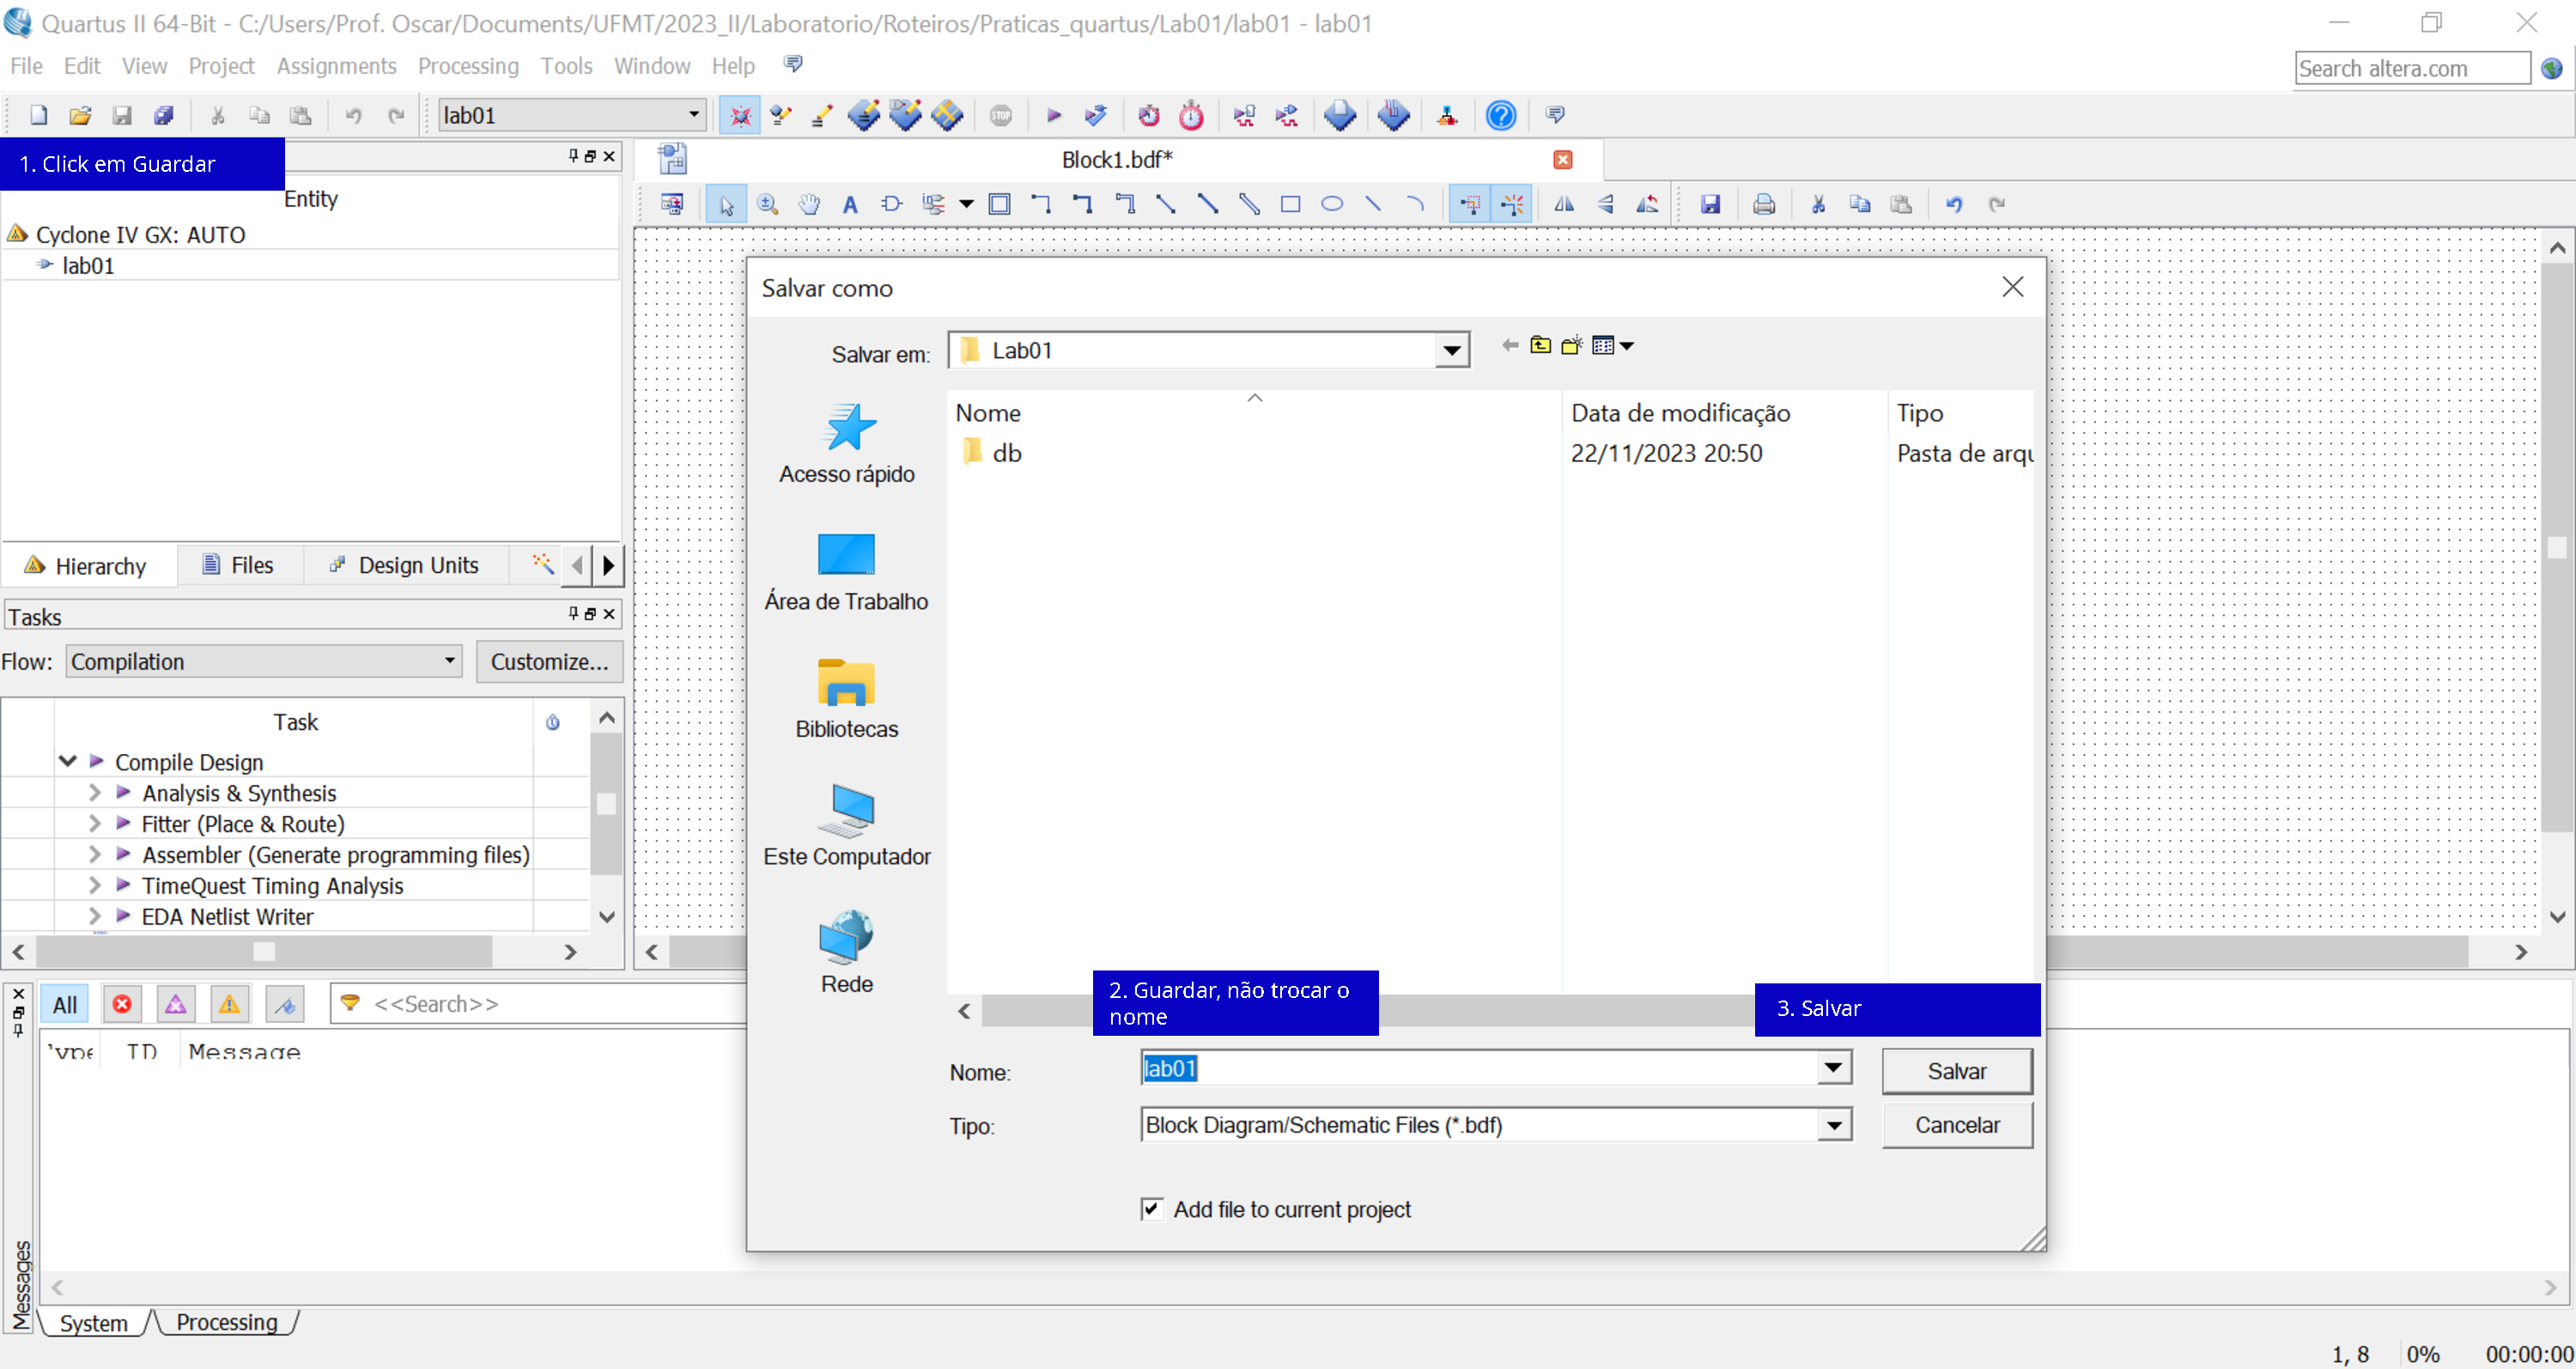
\includegraphics[width=0.45\textwidth]{Figs/fig11.png}
	\end{figure}
	
	
\end{frame}
%%==============================================================================================================
\section{FPGA}
%%==============================================================================================================
\begin{frame}{Field Programmable Gate Array (FPGA)}
	\justifying
	

	
	\begin{block}{}
		\justifying
		Um FPGA consiste em uma matriz de blocos de lógica programáveis (ou elementos lógicos) e uma rede de interconexão programável que pode ser usada para conectar qualquer elemento lógico a qualquer outro elemento lógico. Cada bloco lógico contem circuitos para implementar circuitos lógicos combinacionais arbitrários, além de um D-Flip-Flop e um multiplexador para direcionamento de sinal. 
		
	\end{block}	

		
	\begin{block}{}
	\justifying
	Em contraste com ASICs (Application-Specific Integrated Circuits), os FPGAs oferecem flexibilidade, permitindo que os usuários configurem a funcionalidade do hardware conforme necessário.
	
	\end{block}			

\end{frame}
%%==============================================================================================================

%%==============================================================================================================
\begin{frame}{Field Programmable Gate Array (FPGA)}
	\justifying

	\begin{block}{Arquitetura}
		\justifying
		\begin{itemize}
			\item Composta por uma matriz de blocos de lógica configurável (CLBs) e uma rede de interconexão programável.
			\item CLBs contêm LUTs (Look-Up Tables), flip-flops, multiplexadores e outros elementos essenciais para implementar lógica combinacional e sequencial.
			\item A rede de roteamento permite conectar os CLBs para criar circuitos personalizados.
		\end{itemize}
		
	\end{block}	
	
\end{frame}
%%==============================================================================================================

%%==============================================================================================================
\begin{frame}{Field Programmable Gate Array (FPGA)}
	\justifying
	
	\begin{block}{Programação}
		\justifying
		\begin{itemize}
			\item A configuração do FPGA é armazenada em uma memória SRAM volátil.
			\item A programação em campo (field-programmability) permite atualizações e modificações de hardware mesmo após a fabricação.
		\end{itemize}
		
	\end{block}		
	
	
	\begin{block}{Aplicações}
		\justifying
		\begin{itemize}
			\item Usado em uma variedade de aplicações, incluindo processamento de sinais digitais, comunicação, computação de alto desempenho, controle industrial, e muito mais.
			\item Amplamente adotado em prototipagem rápida, design de sistemas embarcados e prototipagem de ASICs.
		\end{itemize}
		
	\end{block}		
	
\end{frame}
%%==============================================================================================================

%%==============================================================================================================
\begin{frame}{Field Programmable Gate Array (FPGA)}
	\justifying
	
	\begin{block}{Vantagens}
		\justifying
		\begin{itemize}
			\item Flexibilidade e reconfigurabilidade.
			\item Custos mais baixos em comparação com ASICs.
			\item Consumo de energia potencialmente maior do que soluções ASIC.
		\end{itemize}
		
	\end{block}			
	

\end{frame}
%%==============================================================================================================







%%==============================================================================================================
\begin{frame}{Field Programmable Gate Array (FPGA)}
	\justifying
	
	\begin{figure}[h]
		\centering
		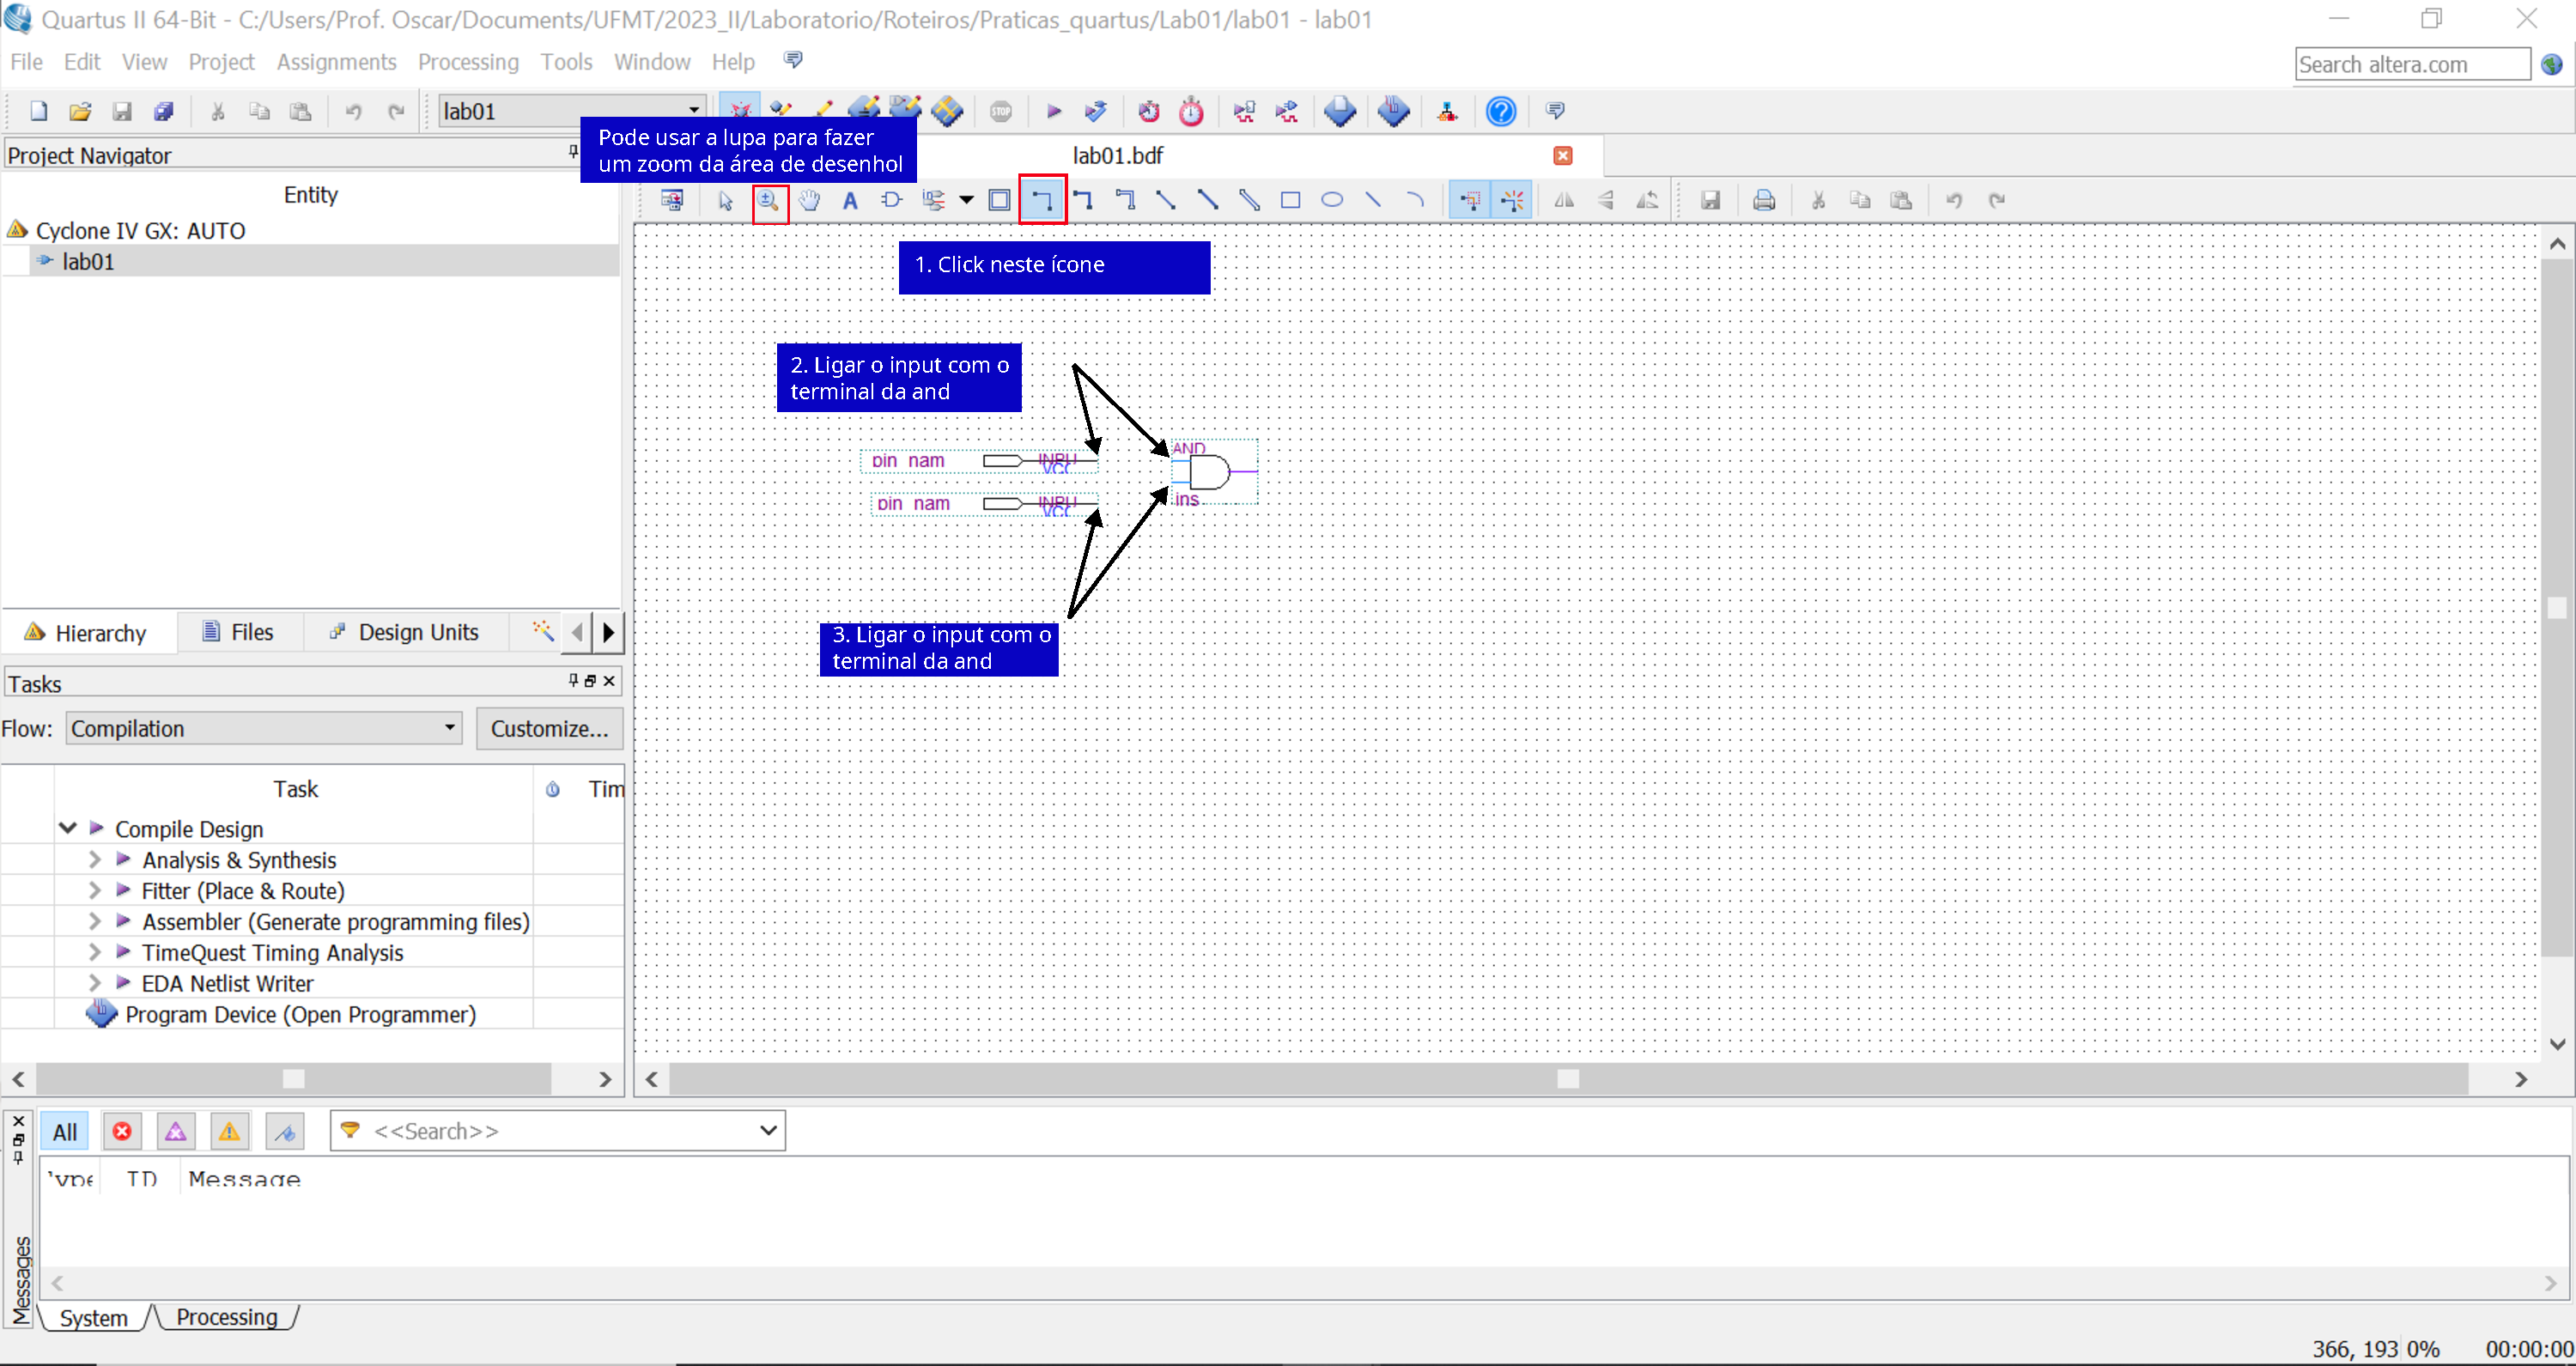
\includegraphics[width=0.42\textwidth]{Figs/fig12.png}
	\end{figure}	

\end{frame}
%%==============================================================================================================

%%==============================================================================================================
\begin{frame}{System-on-Chip FPGA}
	\justifying
	
	\begin{block}{SoC-FPGA}
		\justifying
		É uma integração de um FPGA com uma ou mais unidades de processamento, como um processador de aplicação, processador de sinal digital (DSP) ou processador, em um único chip. Isso combina a flexibilidade de programação do FPGA com o poder de processamento de um processador, permitindo a implementação de sistemas complexos e customizados em um único dispositivo.
		
	\end{block}	
	
\end{frame}
%%==============================================================================================================

%%==============================================================================================================
\begin{frame}{FPGAs hoje}
	\justifying

	\begin{figure}[h]
		\centering
		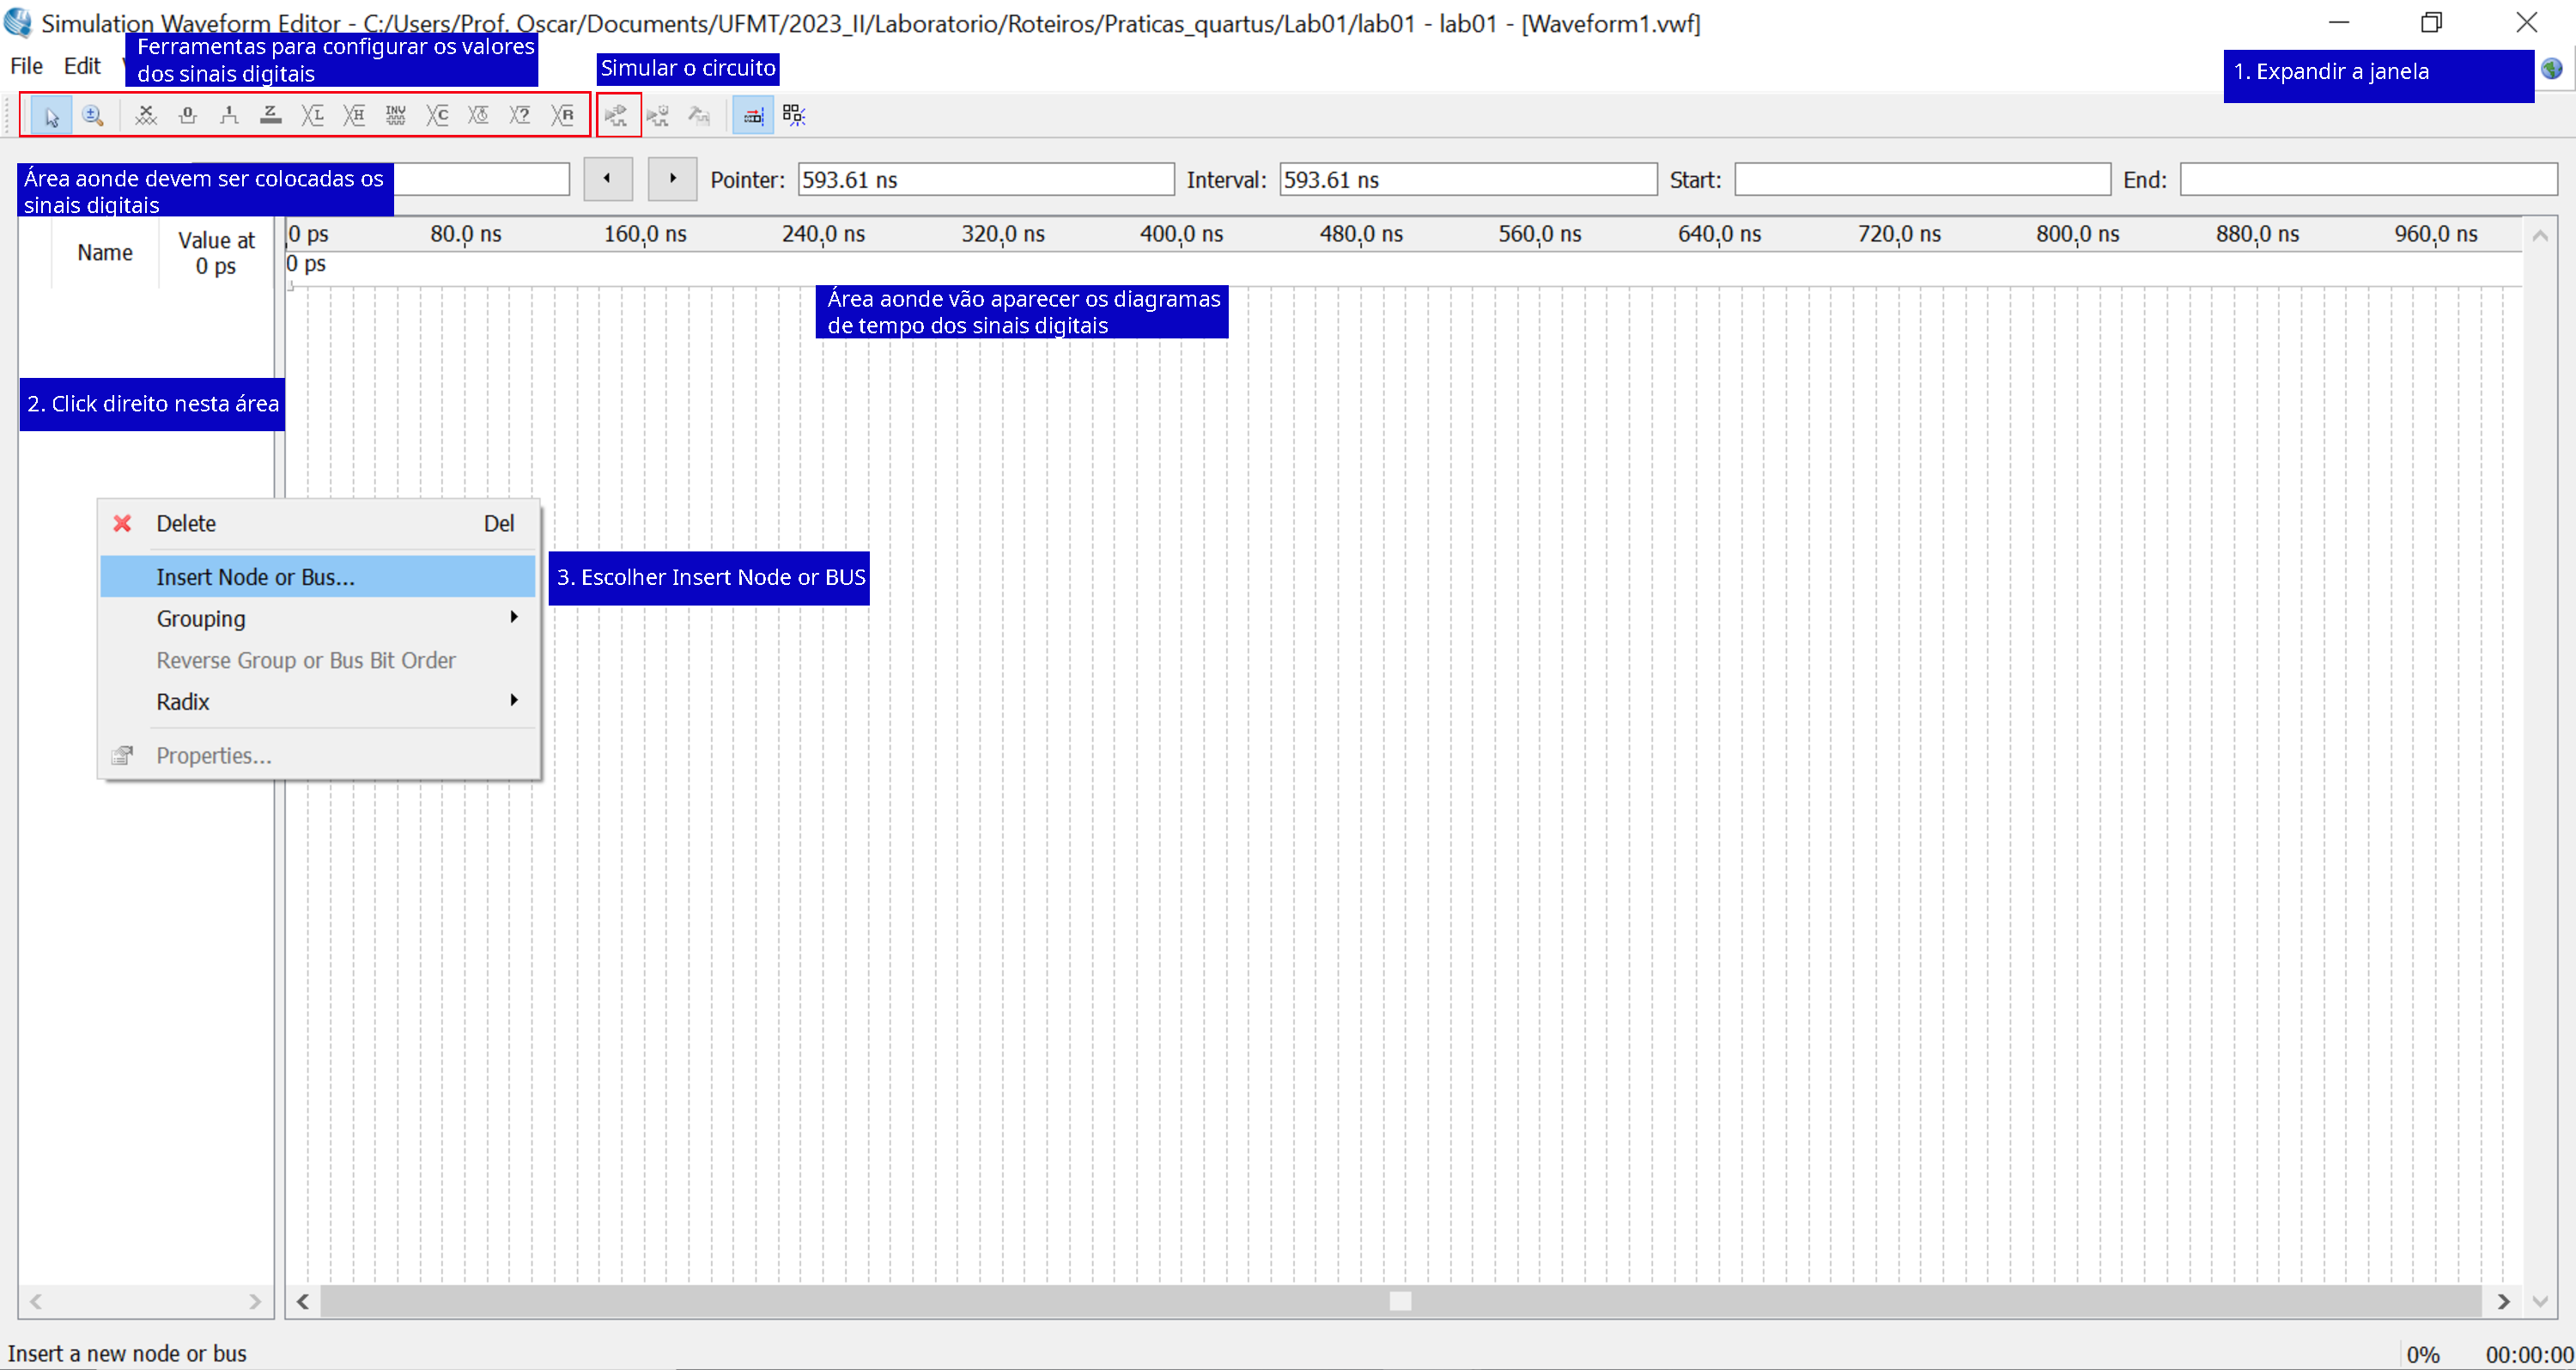
\includegraphics[width=0.8\textwidth]{Figs/fig18.png}
	\end{figure}	
	
\end{frame}
%%==============================================================================================================

%%==============================================================================================================
\begin{frame}{FPGAs hoje}
	\justifying
	
	Intel architecture for the logic part of Stratix 10 and other FPGAs.
	
	\begin{figure}[h]
		\centering
		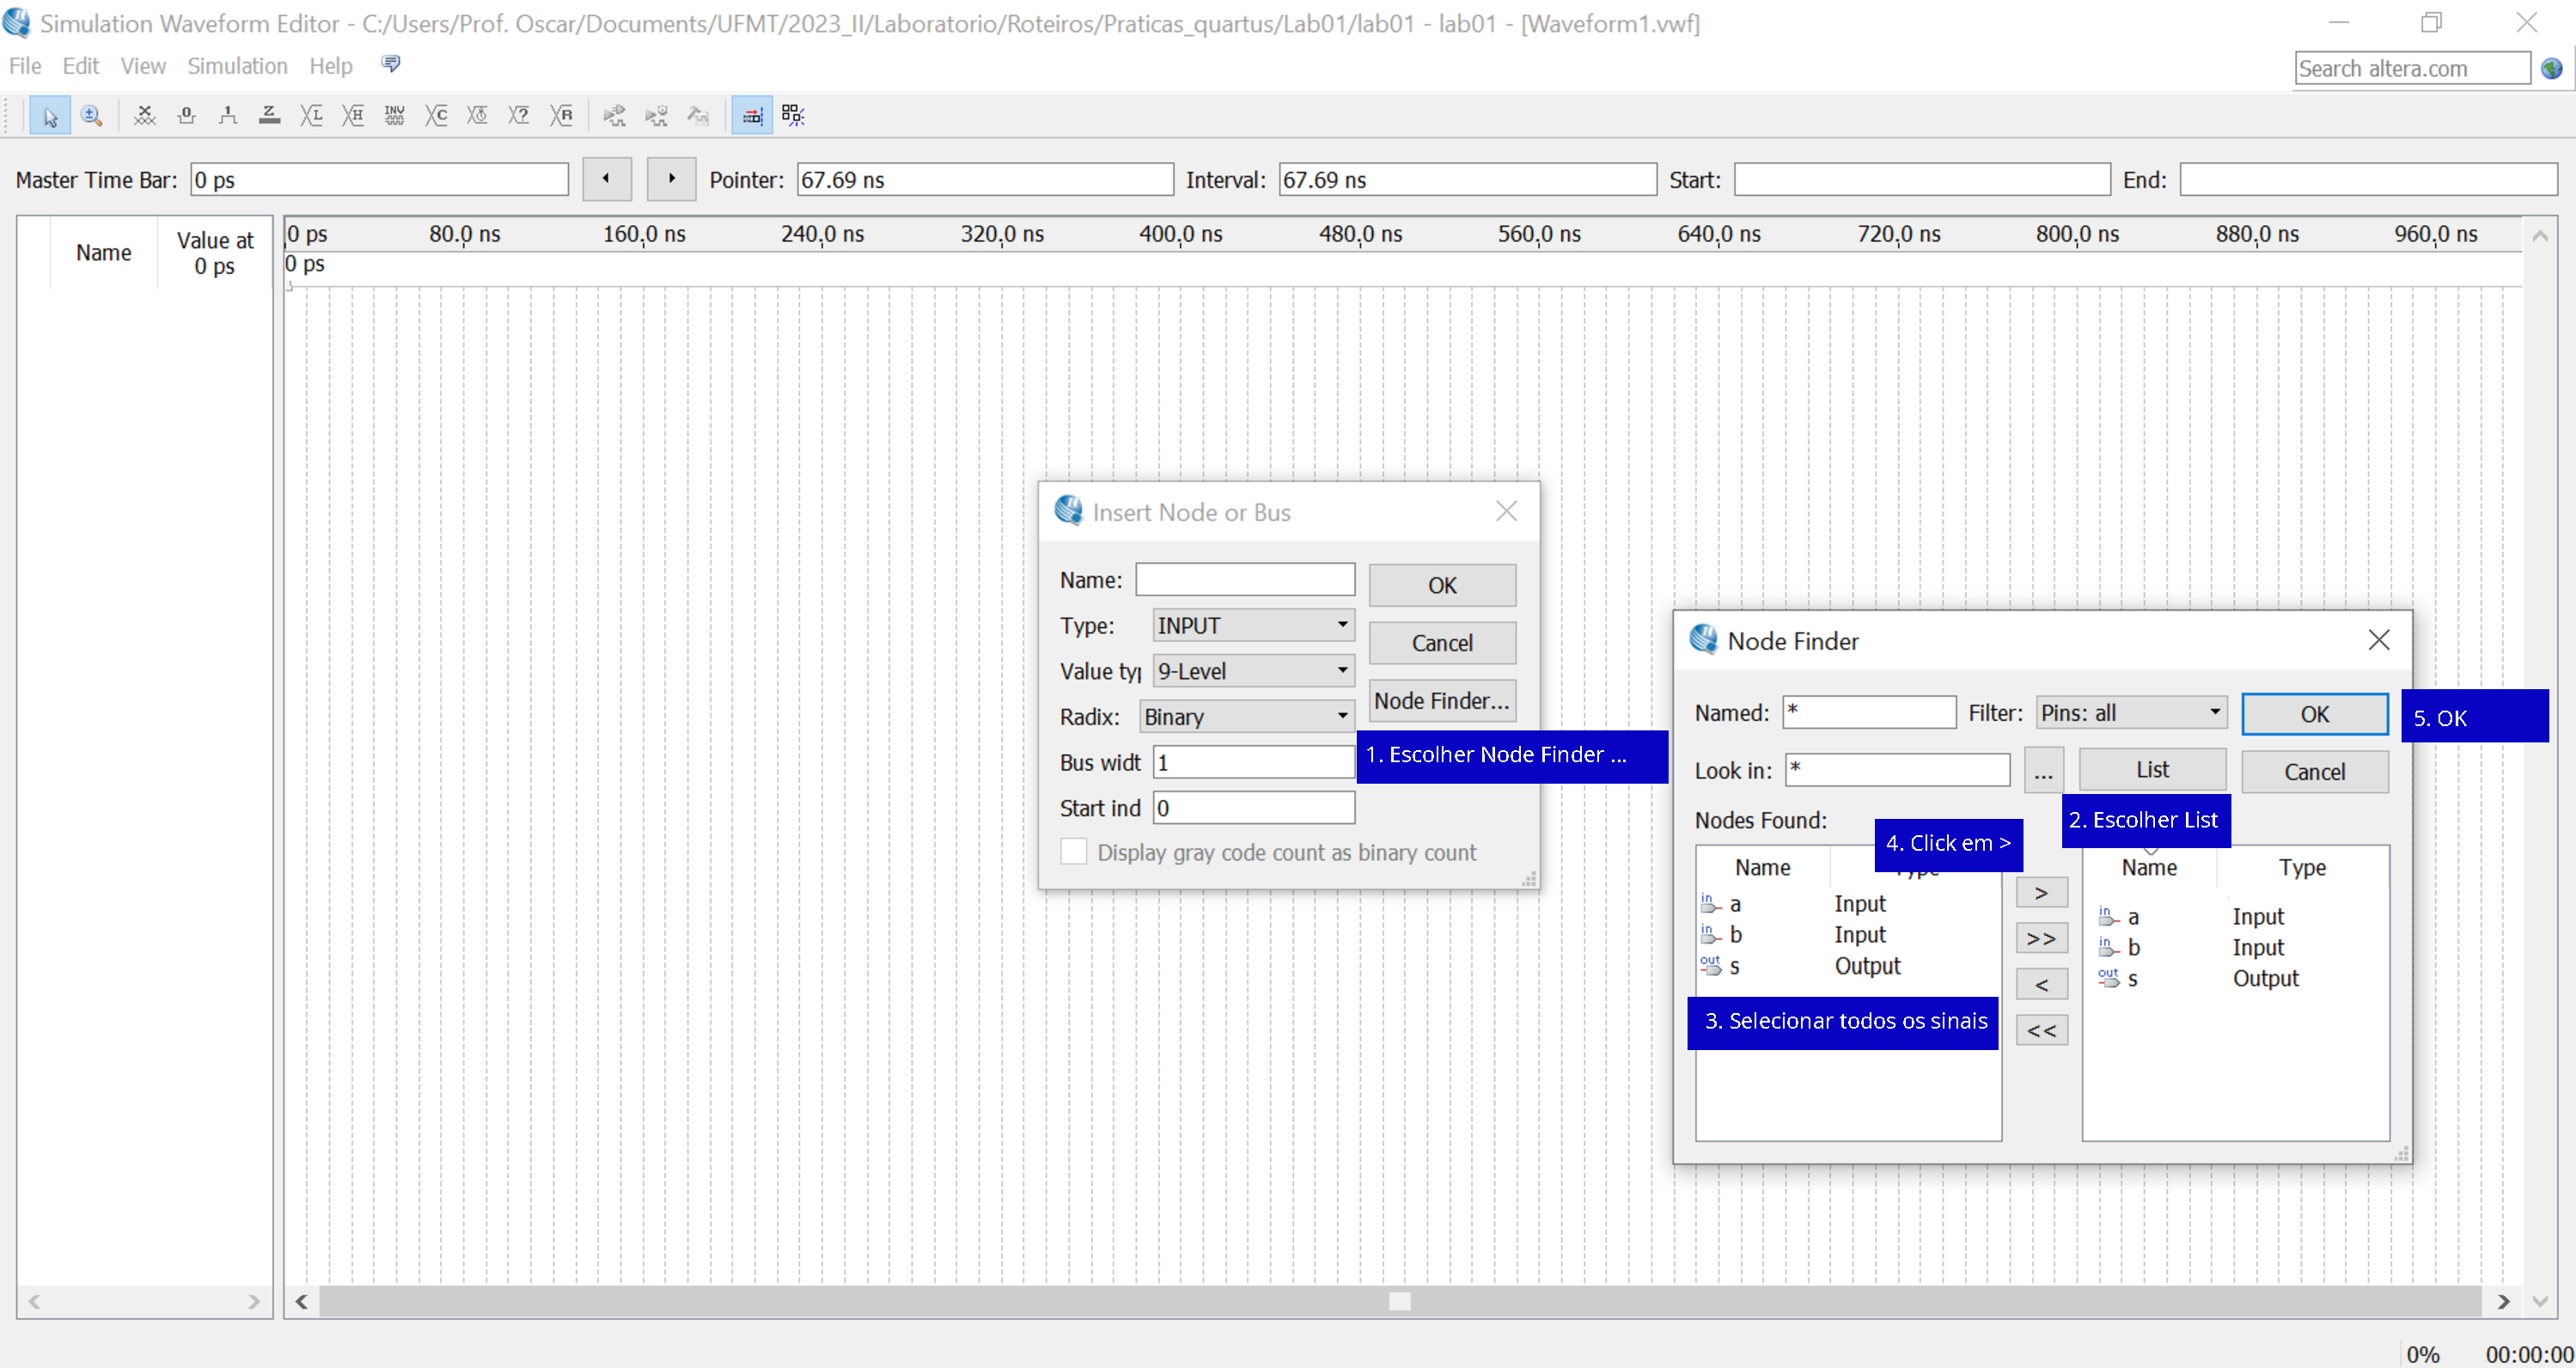
\includegraphics[width=0.8\textwidth]{Figs/fig19.png}
	\end{figure}	
	
\end{frame}
%%==============================================================================================================

%%==============================================================================================================
\begin{frame}{Softcore e Hardcore nos FPGAs}
	\justifying
	
	\begin{block}{Softcore}
		\justifying
		Um processador softcore é um processador que é implementado em uma FPGA por meio de configuração lógica programável. Esses processadores são altamente flexíveis e podem ser facilmente adaptados às necessidades de uma aplicação específica. Exemplos incluem processadores como o NIOS II da Intel (anteriormente Altera) e o MicroBlaze da Xilinx.
		
	\end{block}	
	
	
	\begin{block}{Hardcore}
	\justifying
	Um processador hardcore é um processador que é integrado diretamente na estrutura física do FPGA durante o processo de fabricação. Esses processadores são otimizados para desempenho e eficiência em termos de área e consumo de energia. Geralmente, eles oferecem um desempenho mais previsível e consistente em comparação com os processadores softcore. Exemplos incluem os núcleos ARM Cortex-A9 ou Cortex-A53 encontrados em alguns SoC-FPGAs.
	
	\end{block}		
	
	
\end{frame}

%%==============================================================================================================

%%==============================================================================================================
\begin{frame}{Exemplo de um kit de desenvolvimento}
	\justifying
	
	
	\begin{figure}[h]
		\centering
		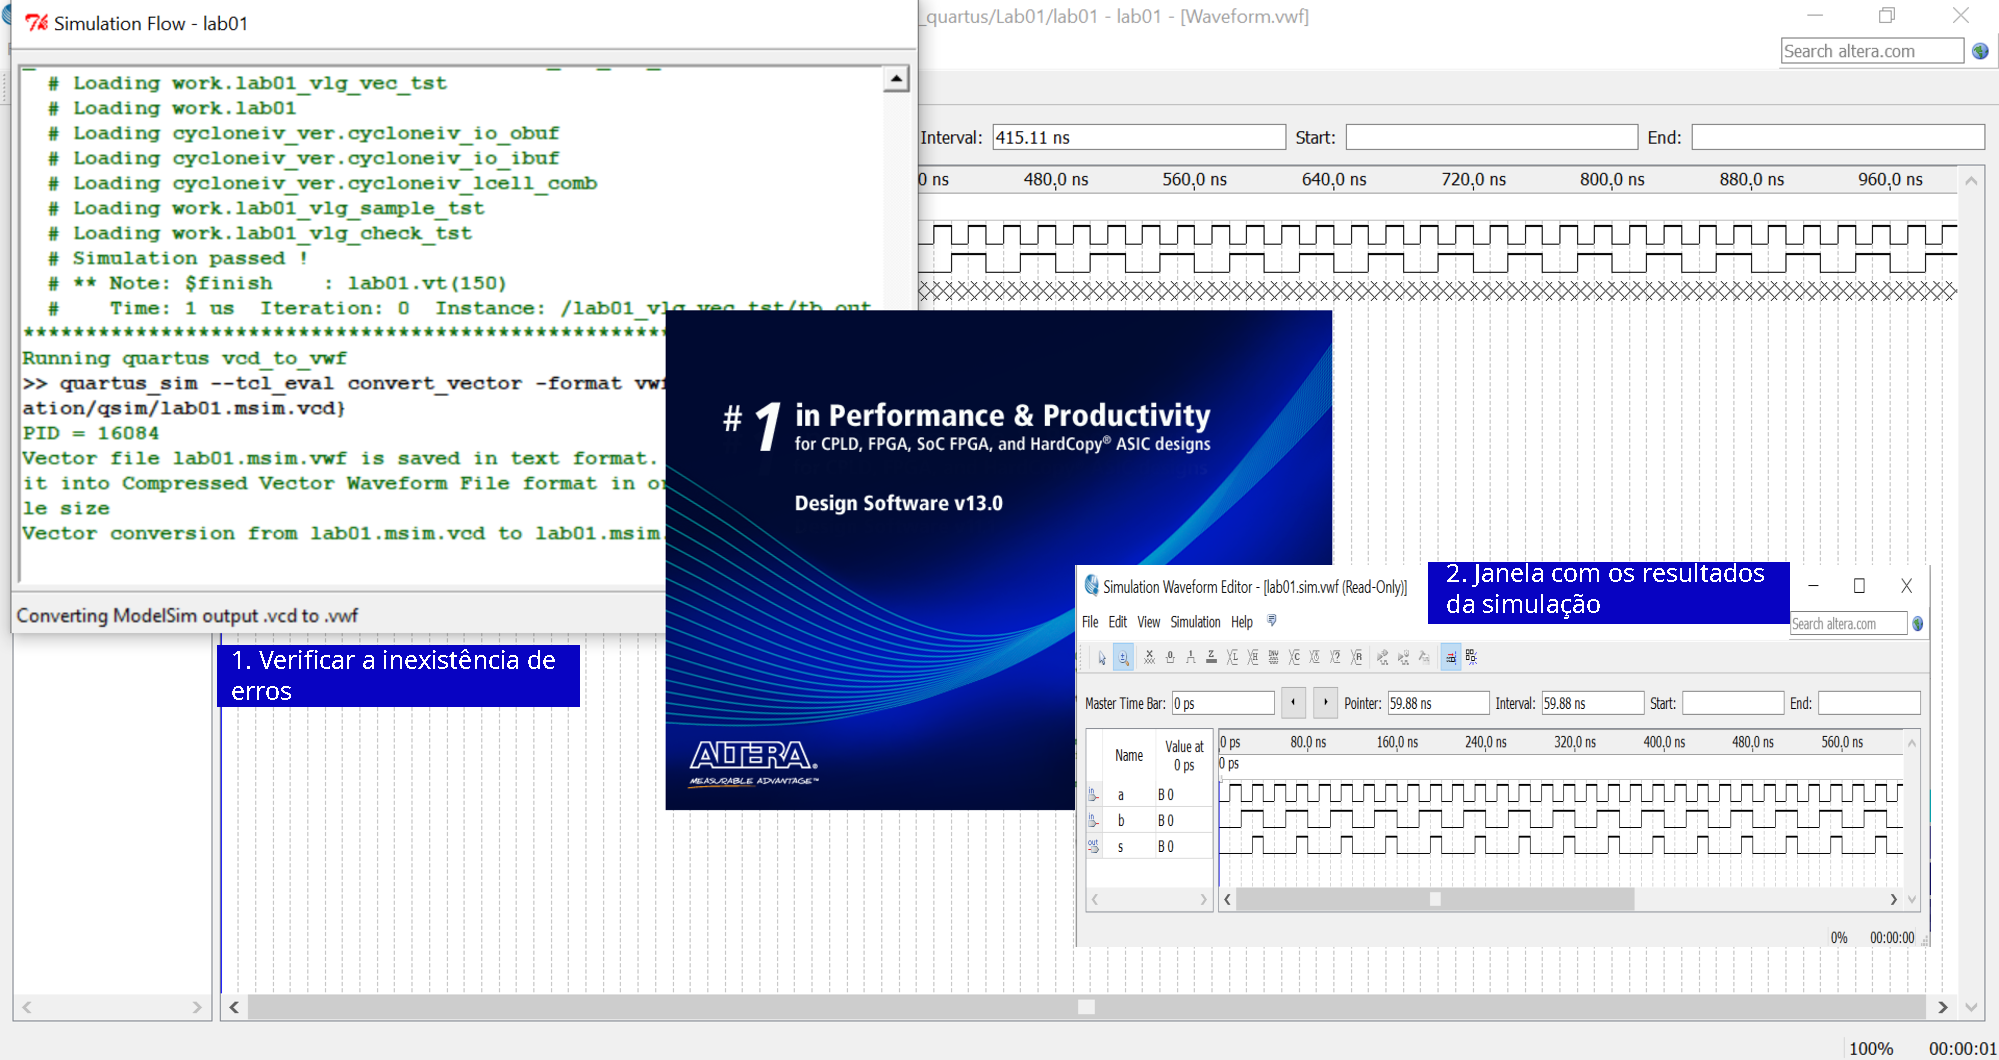
\includegraphics[width=0.8\textwidth]{Figs/fig21.png}
	\end{figure}	
	
\end{frame}
%%==============================================================================================================

%%==============================================================================================================
\begin{frame}{SoCkit}
	\justifying
	
	
	\begin{figure}[h]
		\centering
		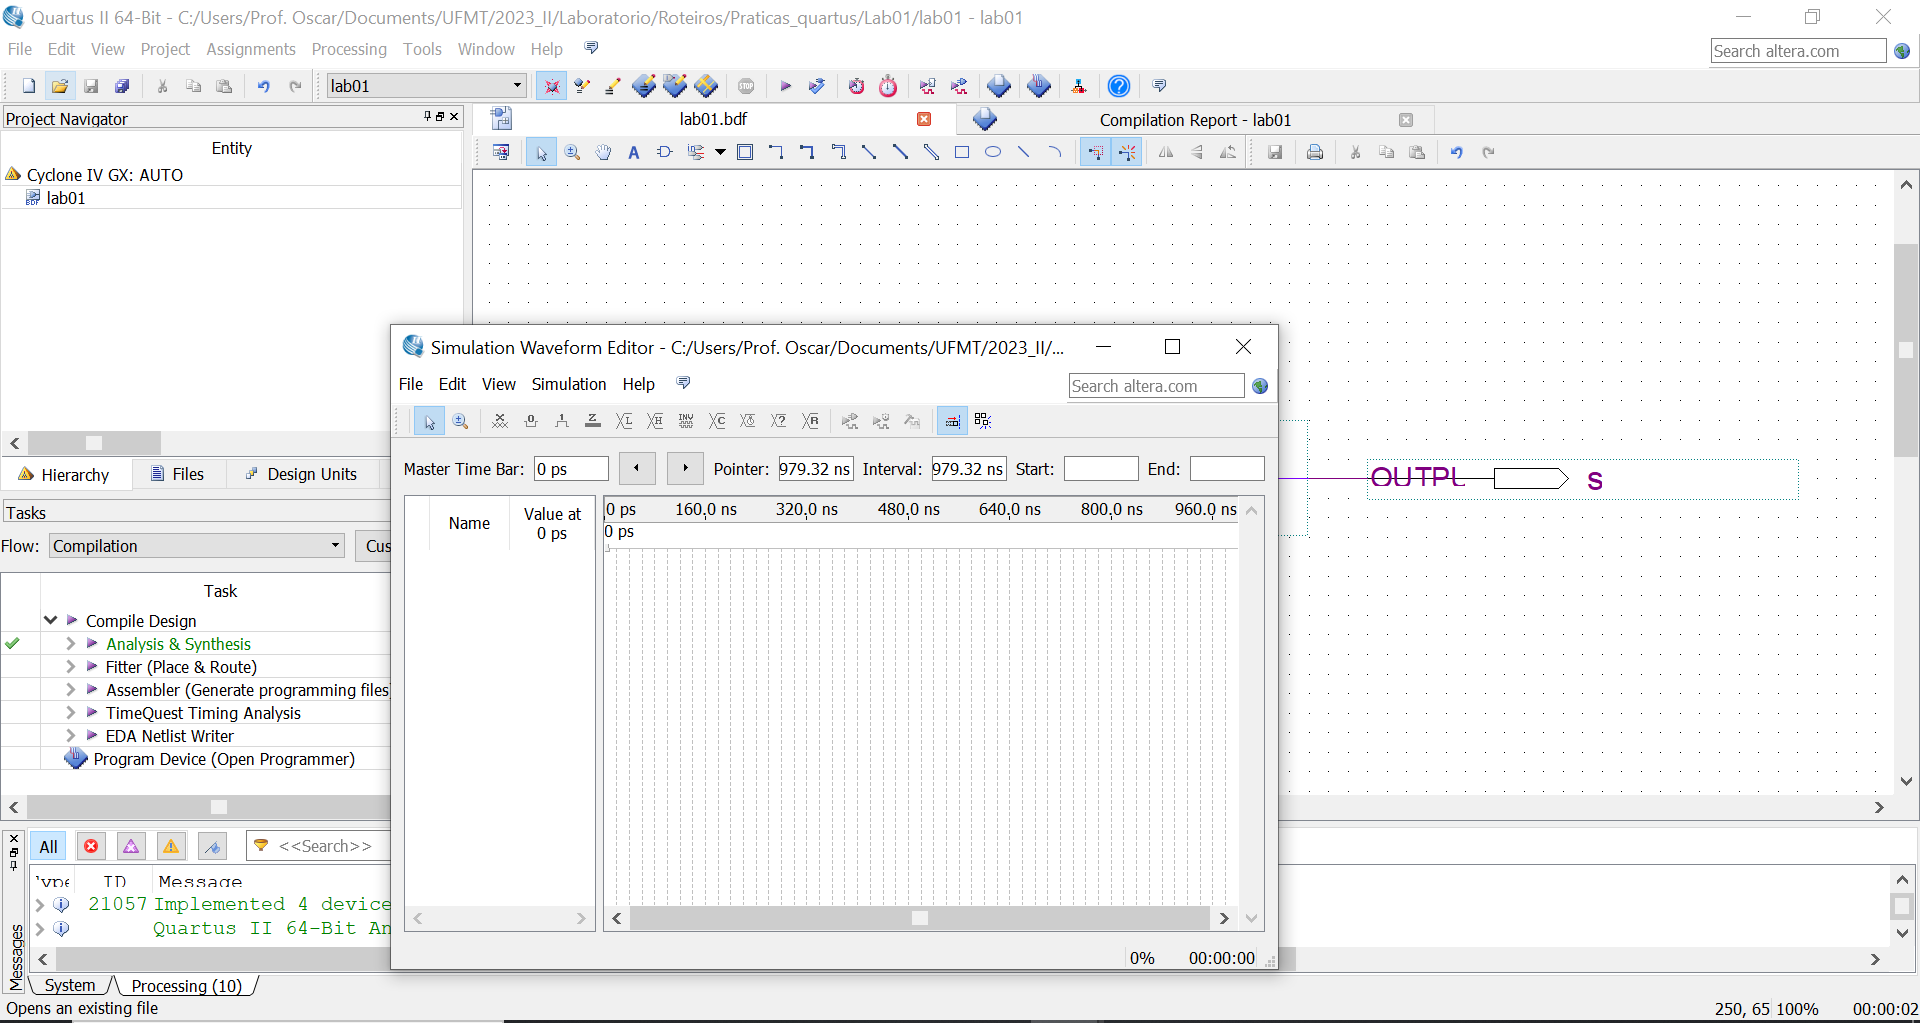
\includegraphics[width=0.62\textwidth]{Figs/fig22.jpg}
	\end{figure}	
	
\end{frame}
%%==============================================================================================================


\section{Aplicação}

%%==============================================================================================================
\begin{frame}{Aplicação}
	\justifying
	
	
	\begin{figure}[h]
		\centering
		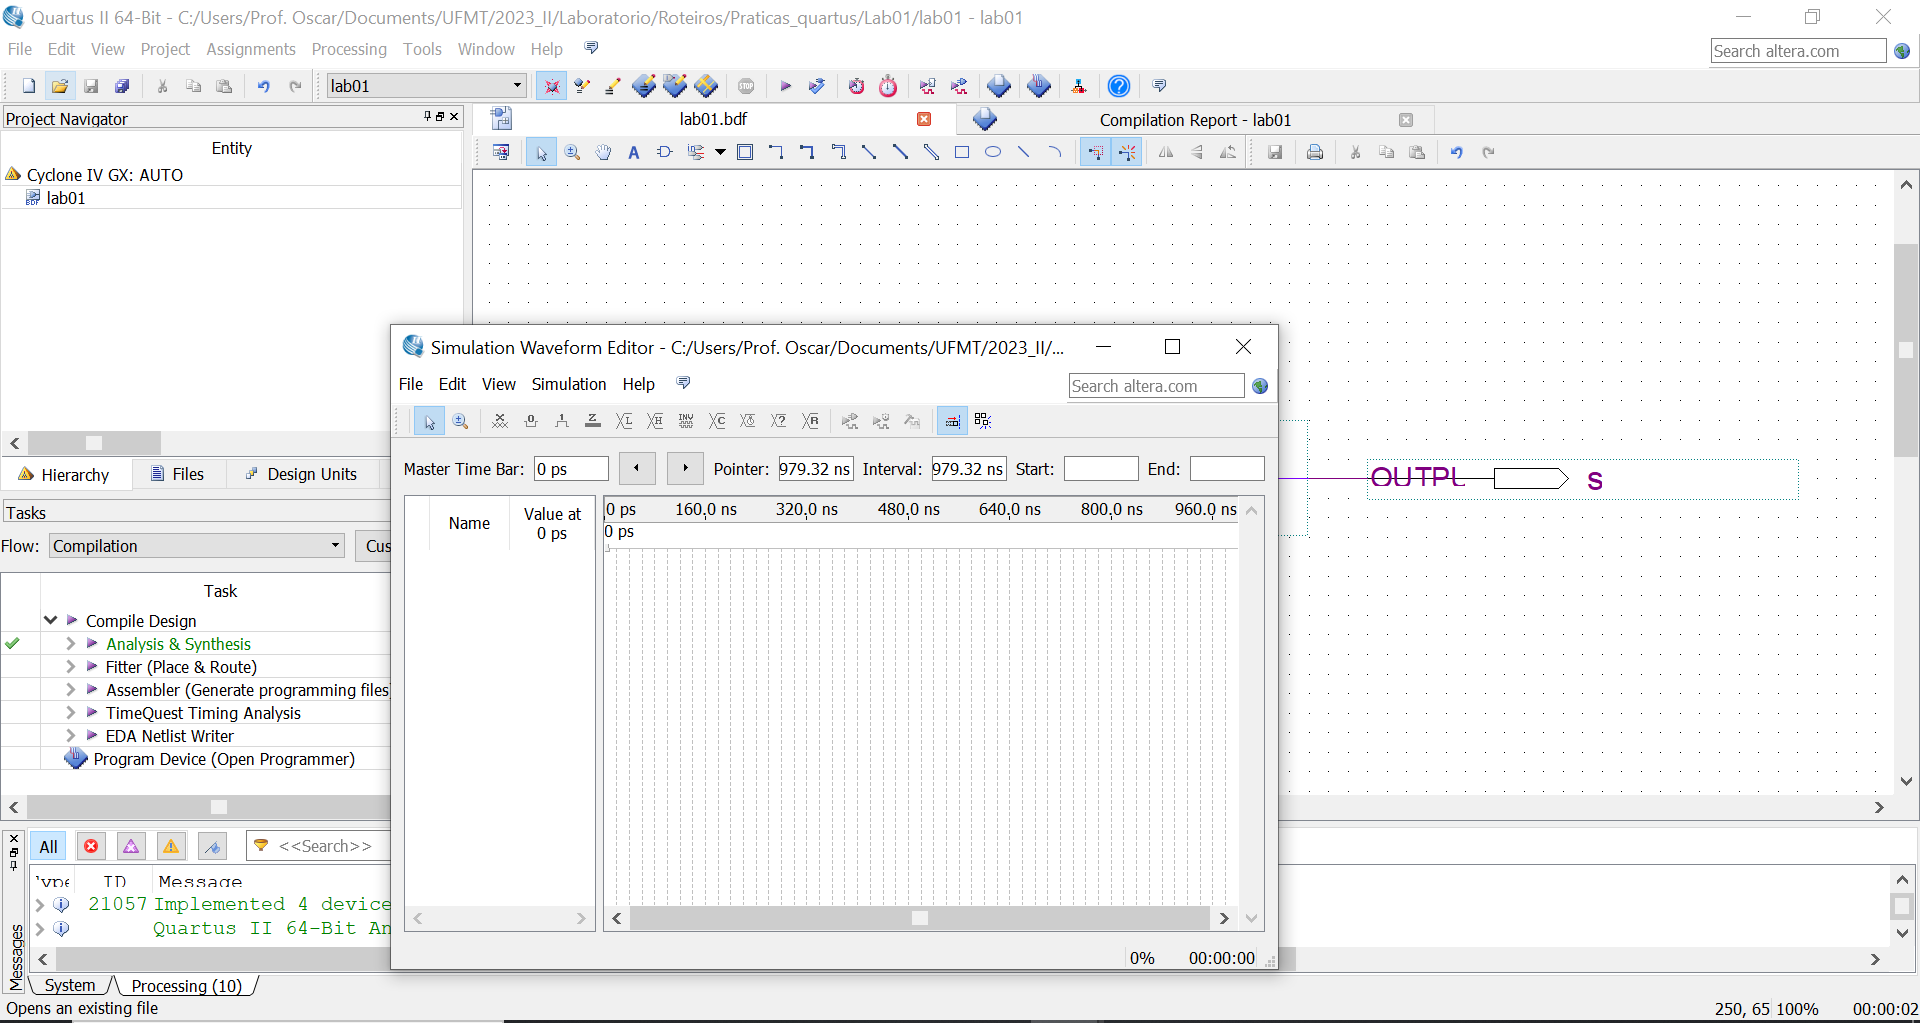
\includegraphics[width=0.7\textwidth]{Figs/fig22.png}
	\end{figure}	
	
\end{frame}
%%==============================================================================================================

\section{DE0-nano}

%%==============================================================================================================
\begin{frame}{FPGA DE0-nano}
	\justifying
	
	
	\begin{figure}[h]
		\centering
		\includegraphics[width=0.6\textwidth]{de0nano/fig01.png}
	\end{figure}	
	
\end{frame}
%%==============================================================================================================

%%==============================================================================================================
\begin{frame}{FPGA DE0-nano}
	\justifying
	
	
	\begin{figure}[h]
		\centering
		\includegraphics[width=0.84\textwidth]{de0nano/fig02.png}
	\end{figure}	
	
\end{frame}
%%==============================================================================================================

%%==============================================================================================================
\begin{frame}{FPGA DE0-nano}
	\justifying
	
	
	\begin{figure}[h]
		\centering
		\includegraphics[width=0.7\textwidth]{de0nano/fig03.png}
	\end{figure}	
	
\end{frame}
%%==============================================================================================================

%%==============================================================================================================
\begin{frame}{FPGA DE0-nano saídas/entradas digitais}
	\justifying
	
	
	\begin{figure}[h]
		\centering
		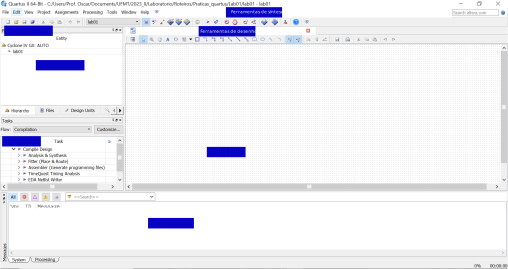
\includegraphics[width=0.8\textwidth]{de0nano/fig04.png}
	\end{figure}	
	
\end{frame}
%%==============================================================================================================

%%==============================================================================================================
\begin{frame}{FPGA DE0-nano alimentação}
	\justifying
	
	
	\begin{figure}[h]
		\centering
		\includegraphics[width=0.8\textwidth]{de0nano/fig05.png}
	\end{figure}	
	
\end{frame}
%%==============================================================================================================


\section{Bibliografia}

%%==============================================================================================================
\begin{frame}{Bibliografia}
	\justifying
	
	\begin{itemize}
		\item Pedroni, V.A. Circuit Design with VHDL. MIT Press, 2004
		\item LaMeres, B. J. (2023). Introduction to Logic Circuits \& Logic Design with VHDL. Suíça: Springer International Publishing.
	\end{itemize}
	
\end{frame}
%%==============================================================================================================


\end{document}
